\chapter{Introduction}
\label{Introduction}

Audio processing, more precisely named audio signal processing, has been of interest since radio broadcasting and telephone systems capable of sound transmission started to replace the morse code \cite{spanias2006audio}. In it's simplest form, as used in the original telegraph, morse code is created by repeatedly opening an electrical circuit manually with a switch so that a visualisation device like a light bulb or an electric bell is turned on and off intermittedly. 


\begin{figure}[H]
    \centering
	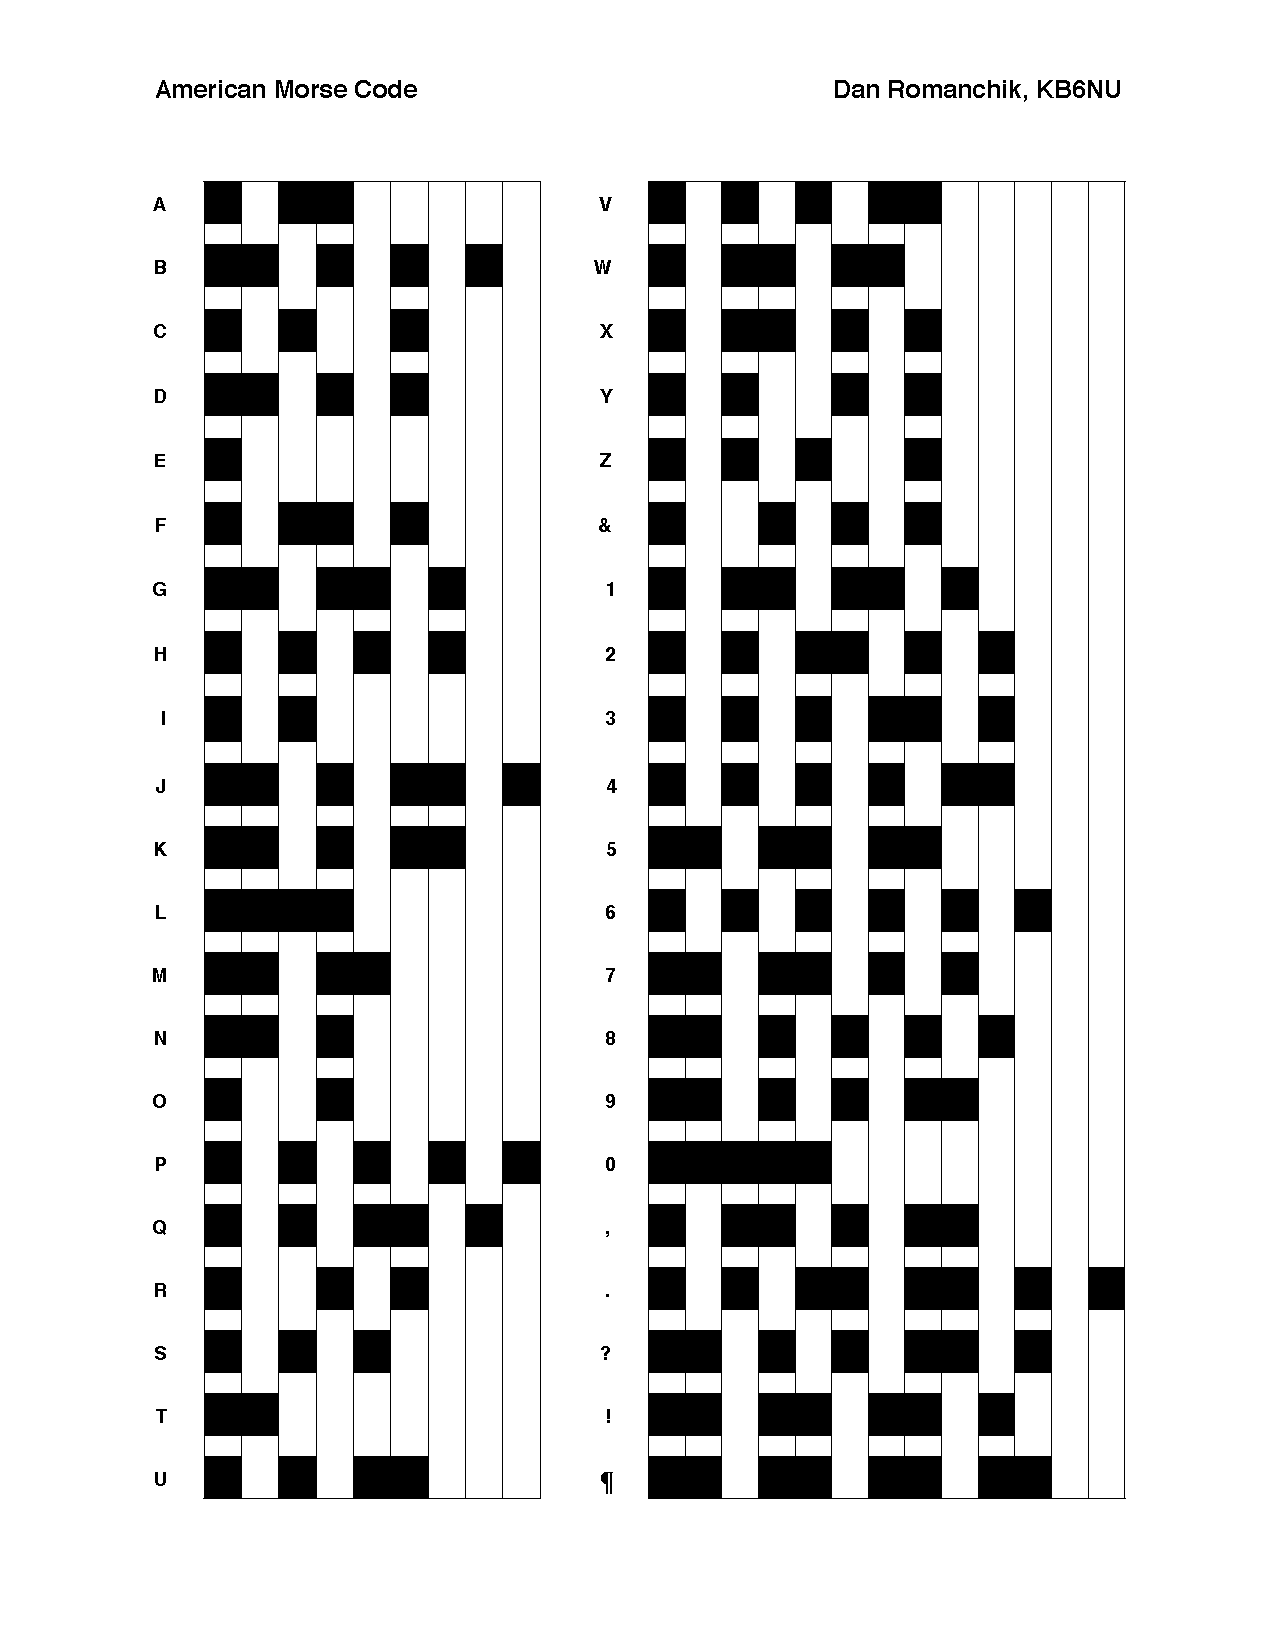
\includegraphics[width=.45\textwidth]{./images/illustrations/morse-chart}
    \caption{A codebook for the international morse code, where black means transmit}
    \label{fig:morse}
\end{figure}

This discrete signal is transmitted over distance by extending the electrical circuit with long wires to a different physical location, so that the switch operator can transmit a message by morse encoding to the recipient who will have to use the same codebook for decoding.

The same purpose can be achieved wirelessly by repeatedly turning a radio transmitter on and off, which can be considered the simplest form of HF-modulation. However, things are more complex for the real- or near-time transmission of speech without manual encoding and decoding. Since most harmonics of the human voice occur in the range of 500 Hz to 2 kHz, according to the Nyquist–Shannon sampling theorem a sampling rate of at least 4 kHz is required for transmission\footnote{To verify this empirically I have downsampled a recording of both my voice and of the rather famous song Tom's Diner to 4kHz. While both the voice and the lyrics were still understandable, the melody perished and the sounds F and S were nearly indistiguishable. This is probably the reason why common speech encoding standards such as GSM's G.711 use a sampling rate of 8 kHz}. When radio transmission was invented in the late 19th century, it was not feasible to encode this information in a digital form (such as morse code). Instead different forms of analog modulation methods had to be developed, which was the birth of audio signal processing.

\begin{figure}[h]
    \centering
	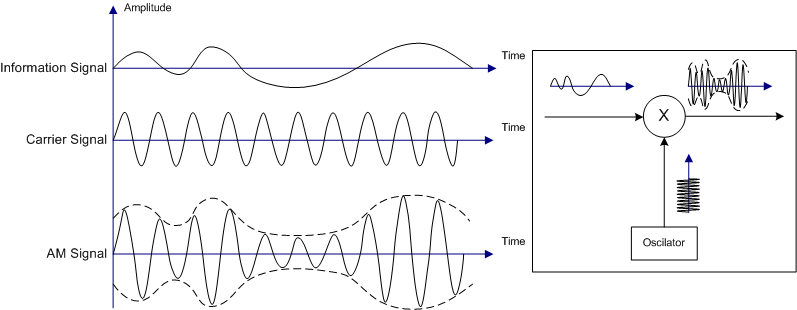
\includegraphics[width=.95\textwidth]{./images/illustrations/am}
    \caption{Amplitude modulation. Created by Ivan Akira. Source: Wikipedia; CC-BY-SA}
    \label{fig:am}
\end{figure}

From the early 20th century onwards it started to transcend its original use while still being required for every form of telecommunication. When home audio playback become available with the phonograph, the analog storage technology necessitated significant frequency alterations to compensate for the mass inertia of the mechanical stylus and diaphragm (so called equalization)\cite{copeland2008manual}. Later the development of cinemas lead to improvements in speaker technology, separation of tweeter and woofer and required the invention of crossover networks \cite{spanias2006audio}.
Today it is widely used for purposes such as entertainment (iPod), medical devices (ultrasound systems), magnetic storage of information (audio cassette, hard disks), and speed measurements  (doppler effect).
 
 
Before computers enabled digital signal processing, audio was transformed through discrete analog circuits. For example, an equalizer might be constructed by using resonant circuits (consisting of an inductor and a capacitor) as frequency filters to allow independent gain control with separate amplifiers for different bands.
There are several different areas of audio processing such as: sound effects, modulation and demodulation, compression, and quality enhancements like noise reduction.

An especially interesting area of audio processing is classification. Given an audio sample, choose the best-fit class for that sample from a finite set of classes.  A common usage is music genre recognition (and other music information retrieval tasks) with the purpose of finding the genre a music sample belongs to. In this thesis my specific focus is on urban sound classification: given an audio sample, choose which class, for example, police sirens, car horns, motorcycle engines or other sounds that occur in natural urban environments the sample belongs to. This problem has several applications such as increasing the safety of self driving cars by detecting the existence and direction of car sirens before the car itself becomes visible or measuring the health impact of different forms of noise on the population.

%% Personal motivation

The idea for this thesis came up during my studies at MIT AgeLab's human factors on traffic research group. At that time the group was working on various traffic safety projects. Human behaviour was first to be recorded in every day traffic by equipping volunteers' cars with cameras. It then had to be analysed by scientists. For large amounts of data this created an enormous amount of work so there was a project that applied computer vision technologies to assist in the creation of situational awareness for the research team and automatically analyse certain situations, e.g. Tesla Autopilot handoff. 


\begin{figure}[h]
    \centering
	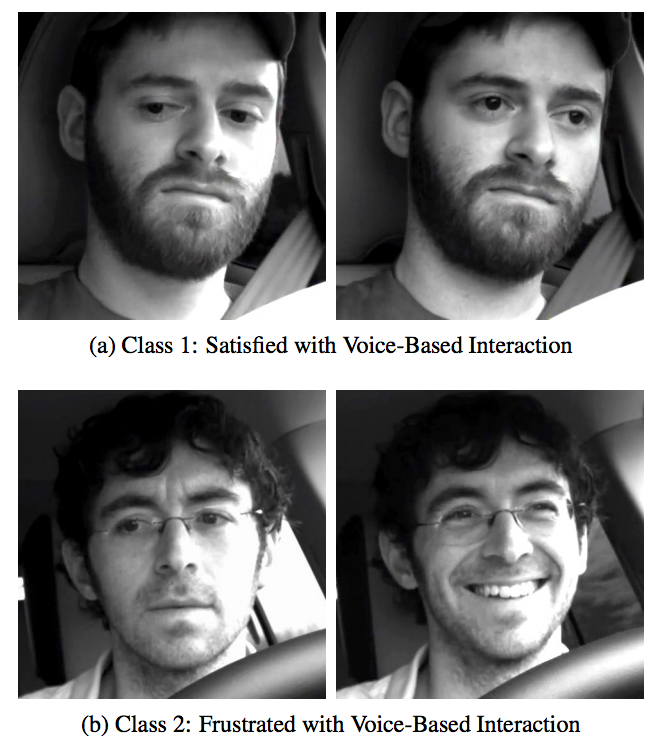
\includegraphics[width=.85\textwidth]{./images/illustrations/driver-frustration}
    \caption{Different examples of concentration and frustration while interacting with an in-car voice control system as shown in \cite{Abdic:2016:DFD:3060621.3060809}.}
    \label{fig:am}
\end{figure}


Just before I started, the team had finished their first paper on using audio detection to annotate road conditions (dry, wet, snow) \cite{Abdic:2016:DFD:3060621.3060809}. This immediately caught my attention as I expected that advanced driver assistance systems and other levels of vehicle automation acoustic detection capabilities might enhance system characteristics in the response to other vehicle and environmental cues. When I did further research I however discovered that research on acoustic machine learning is surprisingly rare apart from speech recognition. This sparked my interest, whether it would be possible to combine audio processing and machine learning for traffic safety purposes. 


%%The first project idea was to assist MIT AgeLab's human factors research in the traffic safety impact of self driving cars. This lab has a long history of detecting different forms of driver frustration with monitoring equipment in cars. They have also published research on the automatic detection of these factors through machine learning on video and audio \cite{Abdic:2016:DFD:3060621.3060809} instead of manual annotation.

Machine learning is especially interesting as an addition to the field of audio processing. Previously this has mainly seen popularity in the audio processing task of speech recognition. While there have been many advances in this area, there has been surprisingly little work in other audio processing tasks, for example, in the detection of urban sounds and background audio classification in general. Until recently, these tasks have been approached using sophisticated, hand-crafted features and algorithms that mostly have existed since the sixties or earlier and were optimised to take advantage of analog hardware. As hardware advanced, more modern algorithms and techniques were able to be used such as gradient boosting and neural networks. These approaches represent the current state-of-the-art as it applies to audio classification.



%% WHAT DID NOT MAKE IT INTO THE THESIS
During this project software was created to automatically detect different sounds, most important the Tesla Autopilot's 'immediate takeover alarm`. I also attempted to use the developed detection of car horns to create a geogrpahic dataset of areas with high driver frustration and see if that could be correlated with accident statistics. However the available dataset of recorded traffic audio with position information turned out to be insufficient for this task.

The main purpose of this thesis then was to apply state-of-the-art neural network architectures and feature extraction to the task of urban sound classification using the UrbanSound8K dataset created by J. Salamon, C. Jacoby and J. P. Bello for the Sounds of New York City project \cite{Salamon:UrbanSound:ACMMM:14}. In this regard, I discuss several popular neural network architectures, such as CNNs, LSTMs, and attention mechanisms, and their performance in regards to audio classification. Specifically this thesis explores the use of LSTMs in urban sound classification, both with and without attention mechanisms. Furthermore, the results are compared to the use of gradient boosting and other existing algorithms against the same dataset.

%% Compared to results of the original papers



\chapter{Background and Related Work}
\label{Background and Related Work}

Although there have been some recent breakthroughs in the field by Google's Deep Mind project (\cite{DBLP:journals/corr/OordDZSVGKSK16}) raw audio is rarely used  with machine learning algorithms directly. This is because one minute of mono channel audio, sampled with the very common analog to digital conversion rate of 44.1 kHz, produces the amount of 2.646.000 data points alone. Every single data point is usually stored as a 16 bit integer containing the amplitude of the audio wave at the present moment between zero and the microphones maximum sensitivity, which totals to 42.336.000 bits or roughly 5.2 Megabytes of information per minute of uncompressed mono audio.

%%TODO Check amount of data points

\begin{figure}[h]
    \centering
	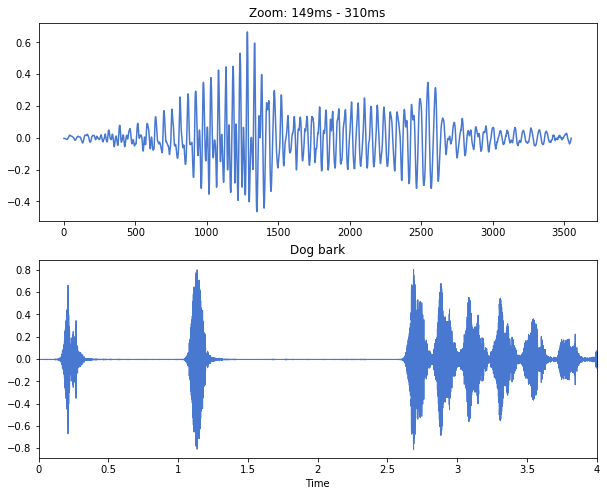
\includegraphics[width=.6\textwidth]{./images/illustrations/audio-signal}
    \caption{Common wave-plot representation of a 4s dog bark audio file and a zoom into seven 23ms frames consisting of 3549 data points}
    \label{fig:audio}
\end{figure}


This is in stark contrast to the amount of data in other machine learning tasks. For example in the very common MNIST image recognition dataset of handwritten numeric digits each image consists  28x28 greyscale pixels which leads to a binary representation of $28*28*8 = 6.272$ bits of information \cite{lecun1998mnist} - a difference of four orders of magnitude.  


\begin{figure}[h]
    \centering
	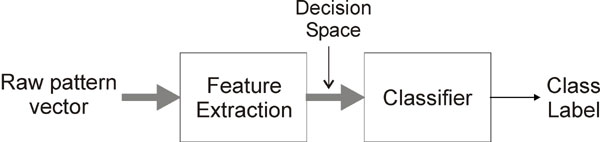
\includegraphics[width=.8\textwidth]{./images/illustrations/pipeline-fe}
    \caption{Source: sheffield.ac.uk - Reproduction under fair use}
    \label{fig:pipeline-fe}
\end{figure}


A common workaround if the amount of data is too big to be efficiently handled directly by classifying algorithms is the technique of feature extraction. This means the creation of signal processing algorithms that transform the raw audio signal into meaningful information of lower bandwith. The most obvious way this an be done is by removing redundancies and irrelevancies while presenting the relevant information in as little dimensions as possible. The main challenge when designing these algorithms is the decision of what exactly might be relevant as this differs strongly depending on the context.
As an example, the well-known MP3 compression specifically removes content that can not be heard by the human ear \cite{brandenburg1999mp3}. While that is adequate for digital compression of an audio file without affecting the listeners' impressions, the same effect could very well decrease the detection and classification rate of a machine learning classifier as it might be based on characteristic features different to human sound perception.  


\section{Machine Learning for Audio Through Feature Extraction}


%[wtd list and describe various audio processing task such as sound classification and speech recognition]

% LOOK UP EXAMPLES OF MACHINE LEARNING FOR AUDIO CLASSIFICATION; ABDIC road mositure

%[wtd describe historical approaches to audio classification and audio processing tasks]


%TODO: Google Urban Sound (Background?) Dataset

For the purpose of this thesis, I have evaluated the ESSENTIA audio analysis library \cite{bogdanov:Essentia:ACMMULTIMEDIA13} through its Python language bindings and the librosa audio and music analysis library\cite{BMcFee:librosa}, which is a native python implementation. 
These have been selected as they seem to be the only actively-maintained open-source packages for audio signal processing with sufficient background literature and documentation. 

Later, during research at MIT my supervisor suggested to compare the results to OpenSMILE, which is promoted as the "The Munich Versatile and Fast Open-Source Audio Feature Extractor" \cite{Eyben:2013:RDO:2502081.2502224}. It is developed by a private company in Garching that is a spin off of a former research group led by Prof. Björn Schuller at TUM.

Besides its versatility the main advantage of OpenSMILE seems to be its extreme ease of use for basic tasks through its command line tool "SMILEextract". A simple demo script that extracts some basic features can be created by invoking 

"\texttt{SMILExtract -cfgFileTemplate -configDflt cWaveSource,cFramer,cEnergy}"\footnote{This example taken from the OpenSMILE manual extracts log energy features broken down into separate frequency bands. There are configuration examples for Chroma, MFCC, and PLP features delivered with the library.}.

The resulting csv can be read with a python csv library and very often directly be used for machine learning applications. While this library has proven to be extremely powerful, the  configuration procedure and the multi-step pipeline required a rather complex setup which ultimately led me to prefer librosa. That way the whole process of loading the audio, feature selection and extraction as well at the machine learning steps could be implemented in the same language and easily be demonstrated and debugged using Jupyter Notebooks.

%TODO: Correlation coefficient with results from librosa and OpenSMILE.

\subsection{Spectrograms}

Probably the best-known feature extractor is the Fourier Transformation. In 1822, while studying heat transfer, Joseph Fourier proved that certain functions could be written as a sum of a finite number of harmonics \cite{fourier1878}. This led the way onto the development of the Fourier transform, the decomposition of a signal into the different sine frequenices it is made up of. As input, the Fourier transform requires a periodic and infinite signal. This precondition is unrealistic in real-world scenarios, where this method is employed on recorded instead of generated input data. As a simple workaround the recorded signal is cut into short slices and the transformation is done for each slice individually, with the artificial assumption that the slice would be repeating indefinitely \cite{Smith97}.

The advance of digital signal processing has made it possible to utilise the Fourier transformation method in order to create visual representations of the different frequencies in an input signal such as sound. The most common format of display is a a two-dimensional diagram, where the abscissa represents the time dimension and the ordinate the separate frequency ranges. The prevalence and intensity of each frequency range can either be displayed through the brightness, hue or a combination of both color gradients for each resulting data point. 


\begin{figure}[h]
    \centering
	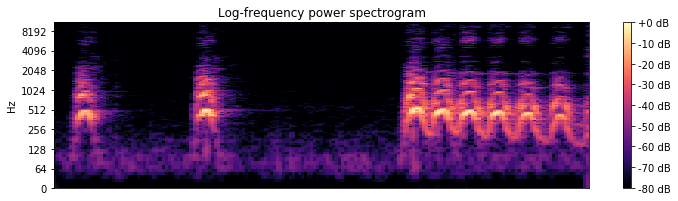
\includegraphics[width=\textwidth]{./images/illustrations/spectrogram}
    \caption{The spectral distribution of the dog bark audio}
    \label{fig:spef}
\end{figure}



To increase verboseness and to reduce the amount of noise, the signal can be smoothed before transformation when individual slices are are not cut but created in an overlapping way through the use of window functions. Subsequently the intensity of each spectrum can be calculated by applying the fourier transform onto the thereby generated individual but overlapping chunks.


\subsection{Mel Frequency Cepstral Coefficients}
\label{MFCC}


\begin{wrapfigure}{r}{0.4\textwidth}
    \centering
	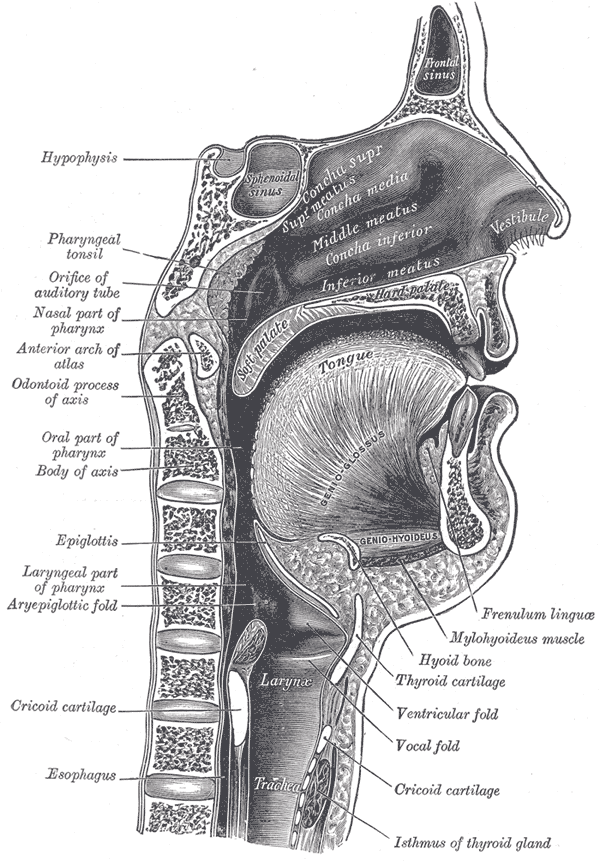
\includegraphics[width=.375\textwidth]{./images/illustrations/Sagittalmouth}
    \caption{Vocal tract in humans - Source: Wikimedia Commons; Copyright expired}
    \label{fig: Sagittalmouth}
\end{wrapfigure}



In Indo-European languages a change of the pitch usually does not alter a spoken word’s meaning \cite{auditoryneuroscience}. Instead information is encoded by filtering the sound while passing the vocal tract, including the pharynx and the tongue causing changes in the envelope of the short time power spectrum. This makes the fourier transformation itself not helpful with speech recognition. Other information, such as the speaker's gender and level of nervousness could possible be extracted nevertheless.

That is why a method has become extremely popular that provides a separation between voice pitch and the formants. Developed by \cite{noll67}, the Mel-frequency cepstral coefficients (MFCCs) have become the most commonly used feature in speech recognition tasks \cite{ganchev2005comparative}, a transformation that is inspired by the inner workings of the cochlea, including the sensory organ of hearing inside the human ear, the Organ of Cortil. 


The first step in its calculation is the slicing into short frames through a window function, mimicking inertia in the organ. Different sound frequencies create resonance in different areas of the cochlea’s narrowing spiral tube, where the wobbling of sensory hair called the stereocilia create nervous impulses.

To identify the different frequencies, the next step is the calculation of a power spectrum through Fourier transformation. This result is a power spectrum on a linear frequency scale, which does not correlate well with the perception of different frequencies in humans \cite{mel}. 

 While low frequencies below 20 Hz can hardly be detected, the effect becomes especially predominant with frequencies over 1 kHz. The transformation from the Hertz- onto the so-called Mel-scale is used as the next step to map the spectrum onto the percieved frequencies. 


\begin{figure}[h]
    \centering
	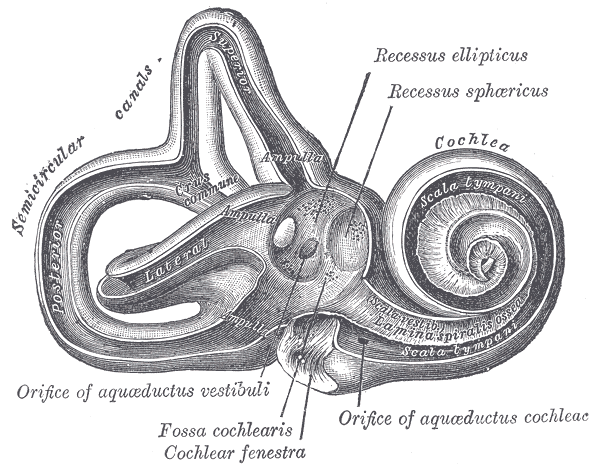
\includegraphics[width=.8\textwidth]{./images/illustrations/Gray921}
    \caption{Location and principle of the cochlea inside the inner ear. - Henry Gray, 1918; Copyright expired}
    \label{fig:gray}
\end{figure}

  
 The linear scale is mapped into discrete bins through a triangular activation functions within the human hearing range as well in this step. Like most human senses in accordance to Fechner’s law \cite{fechner1860} the relationship between stimulus and perception is logarithmic, wich means a quadrupling of the acoustic pressure causes the perceived intensity (loudness) of sound to double. A similar effect can be achieved by taking the logarithms of the power spectrum.

 To decorrelate the energies of the overlapping filterbanks, in order to separate pitch, modulation (added by the vocal in human speech) and noise, usually the discrete cosine transformation is performed on the log mel powers. % The resulting coefficient 2-13 form the MFCCs.
  
  \begin{figure}[h]
    \centering
	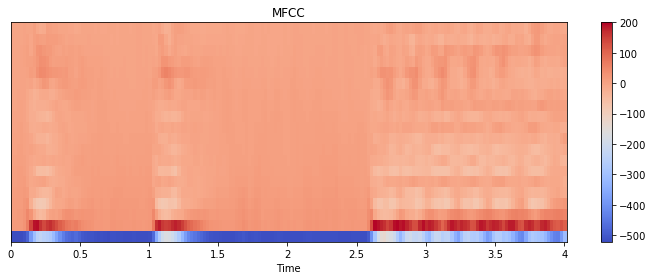
\includegraphics[width=.9\textwidth]{./images/illustrations/mfcc}
    \caption{Graphic representation of MFCCs of the dog bark audio file}
    \label{fig:mfcc}
\end{figure}
 
 The resulting amplitudes form the Mel-frequency cepstral coefficients.

\subsection{Chroma}

The chroma feature is mainly used in music recognition. It is based on the twelve pitch classes commonly used in music theory \cite{Mller:2015:FMP:2815664}. Sounds that differ by one or more octaves, i.e. ratio of frequencies occur at a ratio of $2^n : 1$ with n being an integer are added to the same class.

Image \ref{fig:chroma} illustrates the results of the chroma feature for an audio file of a short concordant clip. Very characteristic for the piano as an instrument is the peak 8 classes above the base class, which can manually be configured as a method of instrument detection. 


\begin{figure}[p]
    \centering
	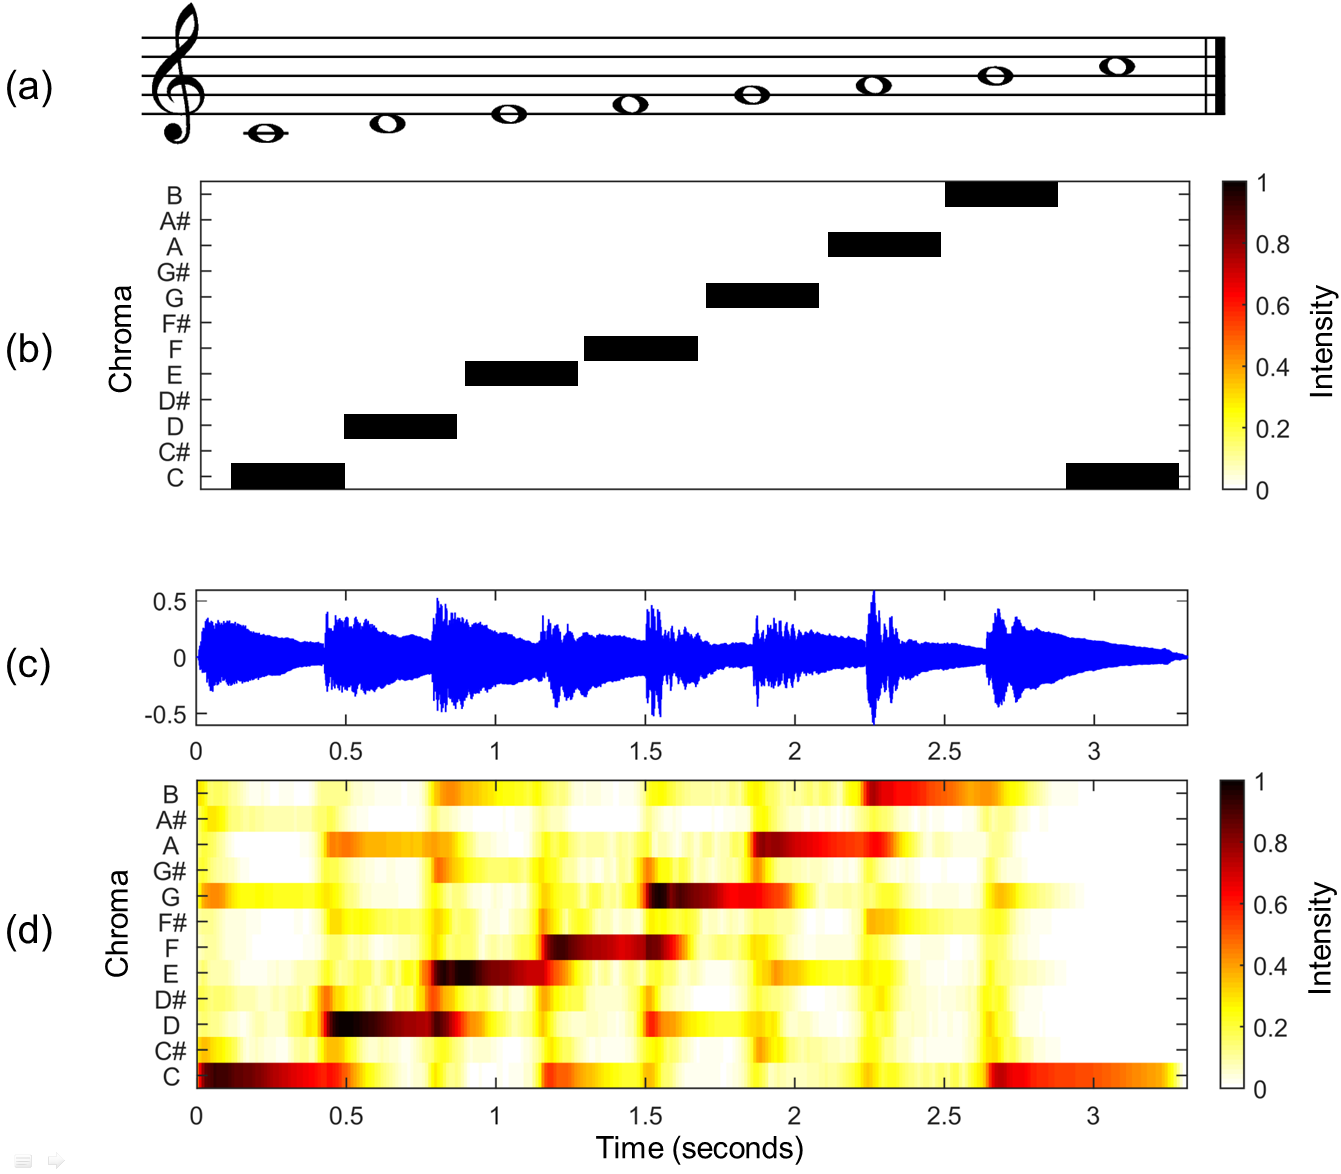
\includegraphics[width=.85\textwidth]{./images/illustrations/chroma}
    \caption{Illustration of the Chroma feature of a C maj scale played on a piano. Created by Meinard Müller. Source: Wikipedia; CC-BY-SA}
    \label{fig:chroma}
\end{figure}



\section{Traditional Machine Learning Approaches}


Machine learning has once more become popular in the last few years as the recent hardware advancements have finally supplied sufficient computational power for training deep neural networks with huge amounts of data.
Mathematically machine learning can easily be described as a system that receives existing data and algorithmically generates a new function that can be used to predict properties of future data.
The quality is measured as the generalisation performance, i.e. the accuracy on data not used for training.

While nowadays there are dozens of different machine learning algorithms known a handful have been found useable for audio information recognition in this thesis.


\subsection{Linear and Logistic Regression}
\label{chptr:reg}

 
The simplest model of a relationship between an explanatory and one dependent variable is the linear regression with a dataset ${\displaystyle \{y_{i},\,x_{i}\}_{i=1}^{n}}$ of n statistical units, with Y being the dependent and x being the explanatory variable.
The model is then calculated based on a linear predictor function where the parameters for slope and intercept are estimated by using the available data.
 
The model is not restricted to a single explanatory variable, where the data set can be described as  ${\displaystyle \{y_{i},\,x_{i1},\ldots ,x_{ip}\}_{i=1}^{n}}$. When multiple explanatory variables are used, the model is referred to as multiple linear regression, where the model will take the form of ${ y_{i} +\varepsilon _{i} =\beta _{0}1+\beta _{1}x_{i1}+\cdots +\beta _{p}x_{ip}}$ with $\varepsilon$ being the error parameter sought to be minimised.

There are multiple ways of estimating the parameters available, with the conditional mean being the most frequently used function, while the median and other statistical qualtiy functions are less common \cite{Yan:2009:LRA:1717831}.  $\varepsilon$ is commonly calculated over the sum of the squared euclidian distances from each Y from the predicted value.


Although simple, multiple linear regression is used extensively for a variety of tasks in practice, for example in Germany to estimate the credit risk of consumers (Schufa) with parameters being the length of the credit histroy, the frequency of address change and the number of different credit cards and bank accounts on one customer. % TODO: Cite


Another generalisation of this concept, where multiple dependent variables are predicted, is the extension of the process called multivariante linear regression. The usefulness of this method is however restricted by the fact that all dependant variables need to be correlated \cite{Yan:2009:LRA:1717831}.


For discrete choice or other distributions where the dependent variable is a discrete or binary category, the modified version called logistic regression was first published by \cite{cox58reg}. Instead of a linear model, the  function ${\displaystyle F(x)={\frac {1}{1+e^{-(\beta _{0}+\beta _{1}x)}}}}$ will always return a value between 0 and 1, that henceforth can be interpreted as the chance of a certain data point falling into the binary category labeled as 1. The same procedure allows us to estimate the relationship of an explanatory variable and the probability of an outcome (e.g. by what percentage would speeding by 10 mph increase the likelihood of an accident).

Parameter estimation is hereby more complicated than in linear regression and an iterative method needs to be used, such as the Newton–Raphson method.

%rule of 10 ?

The primary downfall of linear/logistic regression is the inability to model non-linear relationships. These are very common in nature, famous examples are the half-life of radioactive decay or the exponential growth of most biomass.


\subsection{SVMs}



The so called Support Vector Machine are among the most popular supervised machine learning algorithms and have shown great success in the classification of high-dimensional data. In its simplest form a model is created out of training data, with each instance belonging to one of two categories and the categories are linearly separable.

The biggest improvement in SVMs over more traditional machine learning methods is that it will always find an optimal solution without the risk of being affected by local minima.

\begin{figure}[h]
    \centering
	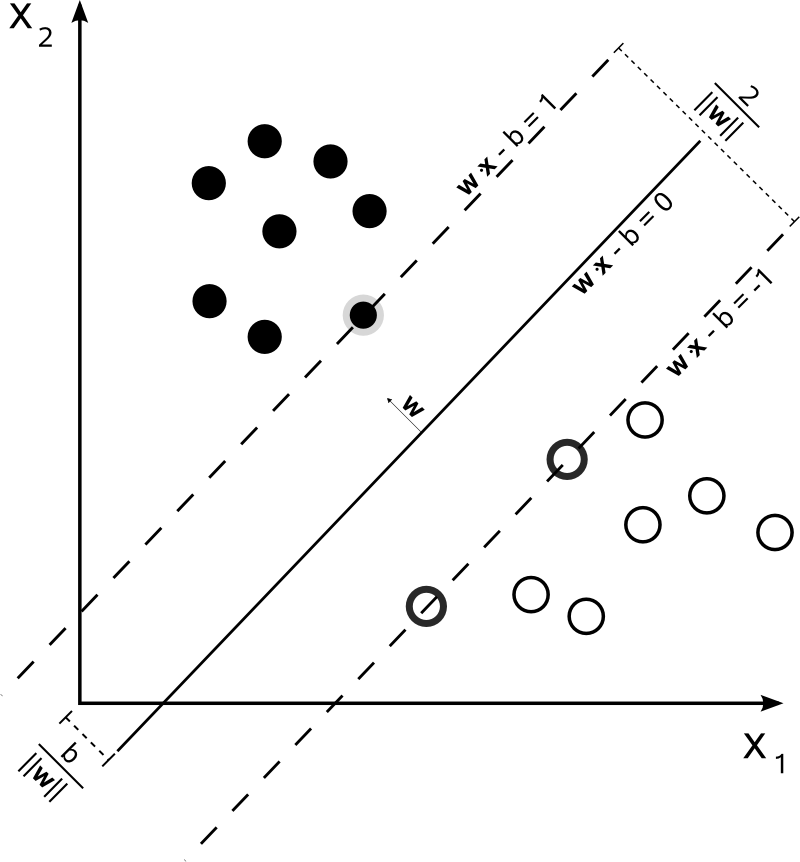
\includegraphics[width=.6\textwidth]{./images/illustrations/svm}
    \caption{Example of linear separation of two classes on maximum-margin hyperplane. Source: Wikimedia Commons; Public Domain}
    \label{fig:svm}
\end{figure}


Support vectors are the subset of all data points lying closest to the decision surface (as seen in figure \ref{fig:svm}). These specify the decision function entirely by themselves. The SVM optimizes the margin around the separating hyperplane (a line in 2 dimensional space) to be maximum.


By using a kernel function, SVMs can be extended onto categories that are not linearly separable. The kernel will transform the original input space that may be non-linear and of higher dimension into a simpler space that can be linearly separated with a hyperplane. Known kernels are available for polynomic, hyperbolic tangent and other relationships. However choosing the right kernel may not always by easy and trial and error with cross validation is sometimes necessary.

Because the hyperplane is known Support Vector Machines can not only be used for classification but also for predictions through regression.


%TODO: citations needed



\subsection{Random Forests}


Random forest classification was introduced with \cite{Breiman2001} and has shown success in multiple rather unexpected areas like medicine, where it was used to predict the development of certain diseases as there are multiple advantages over other classification methods like SVM.

The random forest classifier is a predictive model consisting of a multitude of individual decision trees. The risk of overfitting the model to the available data, but not generalising well to new data is significantly reduced by learning multiple models over different subsamples of the training set and casting a majority vote at prediction time. \cite{statisticallearning}.

The first step in growing a forest is the creation of $n$ random subsamples of the training data, whereby these subsamples are allowed to overlap. Each subsample is subsequently being used to create an independent decision tree, where a small number of features is randomly selected that may be considered as the predictor for each split until the tree is fully developed.

Like other machine learning methods, random forests can be used for regression if instead of decision trees regression trees are computed and the majority vote is replaced with an average over the result of the trees. The performance of using the random forest algorithm for regression however has shown to fall behind other methods and it is therefore seldomly used.

A big advantage of this algorithm is that empirical data from experiments points to the conclusion that the out-of-bag error estimate is almost identical to that obtained by cross-validation, which means it is unlikely that overfitting might have skewed the results. Other advantages are that the evaluation can be parallelised very efficiently through map-reduce, as each tree can be evaluated independently. This makes it very efficient on big amounts of data. Also the training effort only scales linearly with the number of trees, which leads to fast iterations.

These characteristics make random forests useful for audio classification, where the available datasets are usually limited and other algorithms might easily overfit, for example to certain characteristics like the noise profile of the used recording equipment instead of the recorded actual data.

The biggest counterargument to using random forests is that the algorithm was found experimentally and not developed and proven mathematically. That is why its properties are not as well understood as these of many other methods which comes at the price of reduced predictability. Also correct usage seems to be more difficult as programmers tend to optimise the parameters experimentally on the test set and not based on general characteristics of the input data which unintentionally leads to overfitting and a biased validation \cite{StroblMalley}. 

Another part of ongoing discussion is the best practice on the ratio of estimators to features. While the famous publication "How Many Trees in a Random Forest?"(\cite{Oshiro}) concludes a general optimum between 64--128 trees independent of the input's characteristics, the authors' official website\footnote{Link: \url{https://www.stat.berkeley.edu/~breiman/RandomForests/cc_home.htm}} states that "Random forests does not overfit. You can run as many trees as you want" while only increasing the required computational power. Nevertheless, \cite{Segal} has concluded early on that "(the) presence of noise covariates is one factor that can contribute to such profiles". This is a huge caveat when working with audio and requires careful consideration and fine-tuning for our purpose. 

%TODO: higher accuracy on smaller dimensional data or datasets

%TODO: estimators to features 


\subsection{Gradient Boosting}

Gradient boosting is an supervised ensemble learning method that combines many "weak" learners, to form one single strong learner.  It has been proven to be a very successful machine learning method and has been applied with great success to many different challenges of the machine learning competition "Kaggle". Like most methods, it can be applied to both regression and classification problems.

The concept of Adaptive Boosting was introduced with \cite{Freund97adecision-theoretic} and has become the classic example of learning with boosting. It sequentially trains a series of models that are able to accept a weighted collection of training points, i.e. we would add a vector of weights to our training data that indicates the importance of accurately predicting each specific data point. In each sequence the importance of incorrectly predicted data points is increased and the weight of the ones predicted correctly decreaseses and therefore incrementally minimizes the exponential loss.

An unwanted side effect of this boosting technique is that very often the weight of statistical outliers is increased continously and noise is amplified heavily. Adaboost therefor depends on high-quality. % data and experiments during this thesis have not been proven to give useful results TODO: Detail this

The library xgboost \cite{DBLP:journals/corr/ChenG16} has become the de facto standard for gradient boosting after winning Kaggle's Higgs Machine Learning Challenge in 2014 \cite{xgboost-wins}. While there are nowadays bindings for nearly any language available, only the integration into Python's scikit-learn has been evaluated for this thesis.

\newpage

\section{Neural Networks}
\label{nn}


Contrary to the previously discussed approaches to machine learning, neural networks have existed for much longer. Surprisingly, the idea of creating a mathematical model of an artifcial neuron has first been published in 1943 \cite{McCulloch1943} with the intent of studying whether a mammalian brain could truly evaluate computable mathematical functions.



\begin{figure}[h]
    \centering
	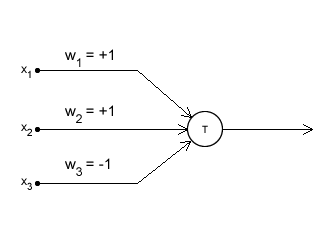
\includegraphics[width=.7\textwidth]{./images/illustrations/mcculloch-pitts}
    \caption{Graphical representation of the McCulloch-Pitts model. Source: aishack.in}
    \label{fig:mcculloch-pitts}
\end{figure}


In this original paper each neuron is a function with one binary output $y \epsilon \{0;1\}$ and one or multiple binary inputs $x_n \epsilon \{0;1\}$ with a specific weight $w_n \epsilon \mathbb{R}$ and a threshold value $T \epsilon \mathbb{R}$. A weighted sum of inputs is calculated, similar to linear regression, with the simple arithmetic operation $\text{sum} = x_1w_1 + x_2w_2 + x_3w_3 + ...$ . The output value is dependent on the neuron's threshold

{\centering
	$y(x_1, ..., x_n) = \begin{cases}
    0,& \text{if } \text{sum} < T\\
    1,& \text{if } \text{sum} \geq T\\
	\end{cases}$
	\par
}

This allows modelling of boolean AND-, OR-, and NOT-relationships, making a network of McCulloug-Pitts neurons a full equivalent to the boolean algebra. Consequently the authors already assumed that nearly every arithmetic function could be calculated with generalisation of this concept form binary in- and outputs to real numbers. This is done in modern neural networks, while also replacing the binary threshold with an activation function (see \ref{activation}).

\begin{wrapfigure}{r}{.5\textwidth}
  \vspace{-10pt}
    \centering
    \hspace{-25pt}
	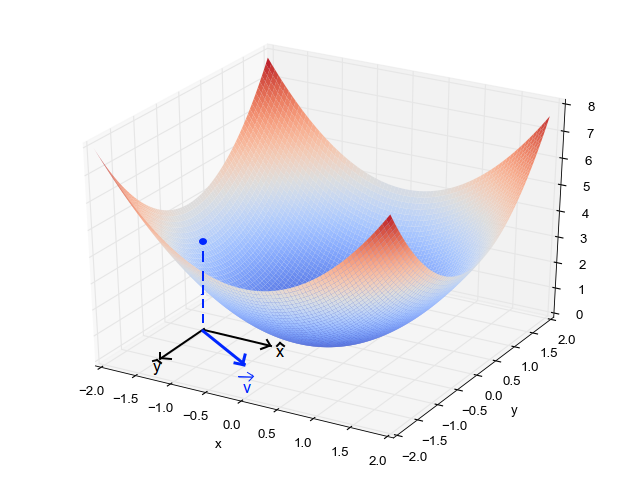
\includegraphics[width=.55\textwidth]{./images/illustrations/gradient-descent}
    \caption{3-dimensional gradient descent\newline Src: Eli Bendersky's website}
    \label{fig:gradient-descent}
      \vspace{-15pt}
\end{wrapfigure}


% explain what neural networks are, put graphs, explain advantages such as ability to deal with curse of dimonsionality and ability to deal with non-linear relationships, explain pitfalls

Another change is the automated learning of weights through methods of stochastic gradient descent, an iterative method of minimising a function by moving the function's input variables along the function's derivative repeatedly. For neural networks this is done on the basis of a cost- (sometimes named "loss-") function which maps the network's classification accuracy onto a real number. 

The first step usually is a random initialisation of all input weights. This will return random output. The error on the training data can then be backpropagated, i.e. the contribution of each neuron to the total error is calculated and the weights are adjusted accordingly.

 %[wtd explain stochastic gradient descent and optimizers ADAM, Adadelta, momentum, etc.]
 

 Neural networks have had a fickle history with an ebb-and-flow of popularity, last peaking in the 90s \cite{Bengio91z}.  Due to advances in computational power, parallel processing paradigms, and neural network architectures in the past several years neural networks are seeing great successes across many machine learning tasks. For example, in \cite{Silver:2016aa} neural networks were for the first time in history able to outperform a human champion in the game of Go, playing at a level previously thought not possible and still leaving many experienced players baffled.  



%The newest branch in machine learning attempting high level abstactions is so called deep learning. 

Tensorflow \cite{tensorflow2015-whitepaper} is a library that was published by Google in 2014 in an effort to open-source their internal deep-learning functionalities into an universal library. While the computational part is written in C++ for performance all functionality, such as designing a network and training the model, is accessed through high-level python bindings in order to simplify the API interface and its implementation in real world use cases. Even though it first lacked distributed computing functionality and the support for GPGPU was poor in the beginning it has rapidly become popular for almost all deep learning tasks and Amazon Web Services\footnote{\url{https://aws.amazon.com/tensorflow/}}, Google\footnote{\url{https://cloud.google.com/ml-engine/}} and nVidia\footnote{\url{https://www.nvidia.com/en-us/gpu-cloud/}} have made hardware accelerated cloud solutions available in the meanwhile.

After a longer trial with Tensorflow, the browser based Convnet.js was evaluated to see if it could be used as a viable alternative for the tasks in this thesis.
Due to its nature of being a JavaScript implementation and the characteristics of any scripted language its performance is obviously unable to match the GPGPU accelerated TensorFlow implementation. It's strength primarily is the web integration which allows to create click-through tutorials and GUIs for demonstration and experimentation that require no primary setup by the end user. 

While the concept is intriguing, the usage in this thesis has not been deemed feasible as the feature extraction still had to be done in a different environment and the subsequent export of the feature vectors and import into the browser has been extremely error-prone. After the trial I have reverted to using Tensorflow while later models were built upon the Keras library (an API frontend that serves as an abstraction layer for multiple neural network frameworks) \cite{chollet2015keras}.



%%TODO: Cite and expand
\newpage

%Hacker's guide to Neural Networks: http://karpathy.github.io/neuralnets/

%GOOGLE CLOUD BIG DATA AND MACHINE LEARNING BLOG - Learn TensorFlow and deep learning, without a Ph.D.: https://cloud.google.com/blog/big-data/2017/01/learn-tensorflow-and-deep-learning-without-a-phd


%WEIGHT INITIALIZATION: https://medium.com/@amarbudhiraja/towards-weight-initialization-in-deep-neural-networks-908d3d9f1e02

%% gradient-based learning methods and backpropagation. In such methods, each of the neural network's weights receives an update proportional to the gradient of the error function with respect to the current weight in each iteration of training. Traditional activation functions such as the hyperbolic tangent function have gradients in the range (−1, 1), and backpropagation computes gradients by the chain rule. This has the effect of multiplying n of these small numbers to compute gradients of the "front" layers in an n-layer network, meaning that the gradient (error signal) decreases exponentially with n while the front layers train very slowly.

\subsection{Activation Functions}
\label{activation}

The McCulloch–Pitts neuron discussed in \ref{nn} simply becomes active if the weighted sum of input vales exceeds the specified threshold value. This only allows a binary output for which most contemporary tasks are far too complex. In contrast the concept of an activation function allows a more differentiated output consisting of a real value. After each neuron has calculated the sum of its weighted inputs, in this case the result is inserted into a (usually non-linear) mathematical function that can perform amplification as well as delimiting, such as \texttt{tanh}, \texttt{relu} or \texttt{softplus}.


\begin{figure}[h]
    \centering
	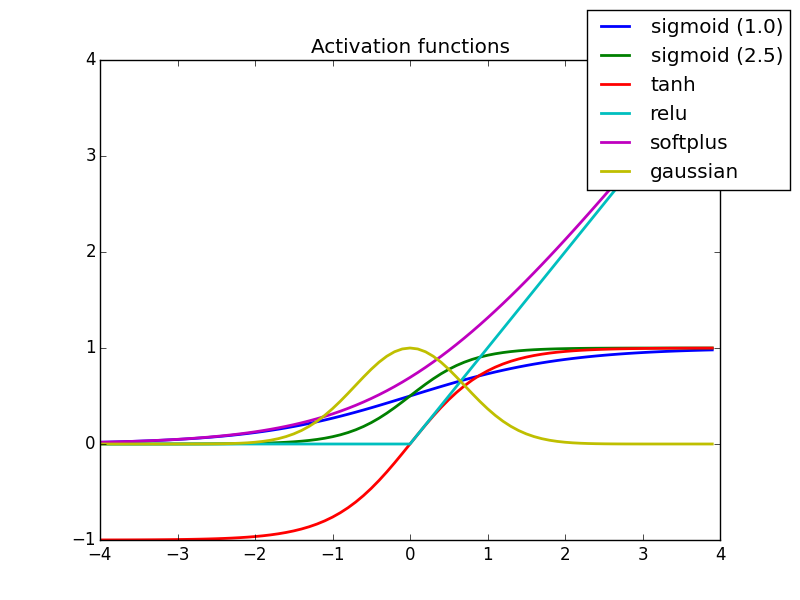
\includegraphics[width=.9\textwidth]{./images/illustrations/ActivationFunctions}
    \caption{Common non-linear activation functions. Source: orngunnarsson.blogspot.de}
    \label{fig:actviation}
\end{figure}

There are advantages and disadvantages to different activation functions and the best fit has to be determined based on the task on hand, the properties of the input and output data, and the available computational power. Sometimes there might not even be a best practice and we have to revert to trial and error.
However, a lot of the recent algorithmic advancements have been made in this area what makes it especially interestring for further consideration:


\subsubsection{Linear}

A linear activation function takes the weighted, summed inputs to the neuron and multiplies it by a constant, giving the neuron the ability to scale the inputs.

{\centering
  $f(x)=cx$\par
}

If the parameter $c = 1$, this activation function is referred to as the identity function and identical to a McCulloch–Pitts neuron without a threshold.


\subsubsection{Sigmoid}

Sigmoid is a mathematical function where the output is constrained by horizontal asymptotes such as $\displaystyle \lim_{x\to - \infty} f(x) =  0; \lim_{x\to + \infty} f(x) =  1$. This causes a very characteristic plot. 

In machine learning, sigmoid refers to a special case of the logit function also used in logistic regression (see chapter \ref{chptr:reg}) described as:

\vspace{15pt}

{\centering
	$\displaystyle f(x)={\frac {L}{1+e^{-k(x-x_{0})}}}$\par
}

\vspace{15pt}


This function mimics a natural growth process, which generally occurs in three phases: The lag phase, in which growth begins slowly and can usually be approximated linearly, an exponential phase of rapid growth with a following stationary phase where environmental limits first slow  down and then bring the growth to a complete stop.

In artificial ecosystems, such as the petry dish, there is usually a fourth phase called death-phase, where the lack of remaining supplies causes the population to shrink rather rapidly. This phase does not exist in the sigmoid model. 

% WIKIPEDIA: Many natural processes, such as those of complex system learning curves, exhibit a progression from small beginnings that accelerates and approaches a climax over time. When a specific mathematical model is lacking, a sigmoid function is often used.[2]



\subsubsection{TanH}

Like all hyperbolic operations, the Tangens hyperbolicus is a generalization of the trigonometric function onto the complex number space so that $\text{tan}(ix) = i * \text{tanh}(x)$. Similar to the  function above, the TanH-function is constrained by two horizontal asymptotes (a sigmodial or s-shaped function), but the range of output is $(-1; 1)$. The function can be calculated as follows:

{\centering
$\displaystyle \tanh x={\frac {\sinh x}{\cosh x}}={\frac {e^{x}-e^{-x}}{e^{x}+e^{-x}}}$
\par
}

\vspace{20pt}

The bigger output range causes a higher derivate of the activation near  $x=0$ compared to the traditional sigmoid. This solves a common problem with back-propagation when normalized data centered around zero causes the back-propagation algorithm to develop biased gradients and is vulnerable to getting stuck in local minima \cite{LeCun1998}.


\subsubsection{Rectified Linear Unit}

More recent networks often use rectified linear units (ReLUs) as activation function in the hidden layers, introduced in 2000 with motivations in biology \cite{Hahnloser:2000aa}. According to Yann LeCun, it has become the most popular activation function in 2015. The formula is relatively simple, returning zero if the sum of the weighted inputs is negative and identity otherwise: 

{\centering
	$\displaystyle f(x)=max(0, x)$\par
}


An advantage is that with random initialisation only half of the neurons will produce an output other than 0 in the first iteration reducing the computational complexity compared to antisymmetric functions like \texttt{TanH} where every cell will produce an output between -1 and 1.
The main advantage however is that the derivative of the identity function is 1 (differentiation of the sigmoid is in the range of 0 and 0.25). This avoids the problem of vanishing gradients \cite{Hochreiter:01book} during backpropagation. That means, the error gradient of each layer's neurons being computed by the chain rule causes the gradient to decrease exponentially with distance from the output, causing layers closer to the input layer to train more slowly.

% allow more effective training on large datasets in deep and complex networks. 

\subsubsection{Softmax}
The softmax activation function transforms a set of probabilities into a vector of real values in the range [0, 1] that add up to 1. Each value in the vector can be interpreted as the probability of 

{\centering
	$\displaystyle \sigma (\mathbf {z} )_{j}={\frac {e^{z_{j}}}{\sum _{k=1}^{K}e^{z_{k}}}}$
	\par
}


\subsubsection{Scaled Exponential Linear Unit}
\label{selu}


A new concept that was published while I was already researching Urban Sound Classification is Self Normalizing Networks (SNN). While most recent advances are due to  recurrent and convolutional layers, the work in the paper \cite{DBLP:journals/corr/KlambauerUMH17} is mainly aimed at improving the (classic) feed-forward network structure.

SELU is a special variant of the Exponential Linear Unit, a function that has an exponential growth below a certain point ($x = 0$ in this case) and linear growth above. 
 


{\centering
	$\displaystyle \text{selu}(x) = \lambda\ \begin{cases}
    x,& \text{if } x > 0\\
    \alpha e^{x} - \alpha,& \text{if } x\leq 0\\
	\end{cases}$
	\par
}

The parameters $\alpha$ and $\lambda$ are not backpropagated but derived from the distribution of the inputs.
With default values\footnote{
As calculated on pp. 11f of \cite{DBLP:journals/corr/KlambauerUMH17} for inputs with a mean of zero with a standard deviation of one the values are
 \(\alpha \approx 1.67326\) and  \(\lambda \approx 1.0507\) }
the function looks similar to relu. However, if the network is not initialized randomly but the weights are distributed with a standard deviation $\sigma = \frac{1}{\sqrt{n}}$ (n being the size of the input) around the mean $\mu = 0$ neuron activations will converge towards zero mean and unit variance during training \cite{DBLP:journals/corr/KlambauerUMH17}. There are other requirements including a modified dropout technique.

The reference paper has shown tremendous success on common machine learning challenges where simple feed-forward networks withs self-normalisation were able to match or outperform complex network's performances, but not everything could be replicated yet\footnote{A  github repo that contains tutorials and implementations of SNNs as suggested by Klambauer et al and served as inspiration for code developed during this thesis is available at: \url{https://github.com/bioinf-jku/SNNs}}.


\subsection{Convolutional Neural Networks}

%One of the more recent improvements in the reserach of Neural Networks has been the invetion of convolutional layers, where the same form of connections between each cell of two neighouring layers is established, like a filter in a traditional programming. 

%Efforts to train the network with know filters, like the sobel image filter have been largely successful by adding before and after images.  

A special network architecture that has proven to generate best results in image recognition is the Convolutional Neural Network \cite{Lecun98gradient-basedlearning}.
Its difference is the existence of a convolutional layer as the core building block.
Instead of having weighted connections between all the neurons in neighbouring layers the network uses a self-taught filterkernel as parameter. Validation efforts to train the network with know filters, like the sobel image filter by simply supplying before and after images have been largely successful.


\begin{figure}[h]
    \centering
	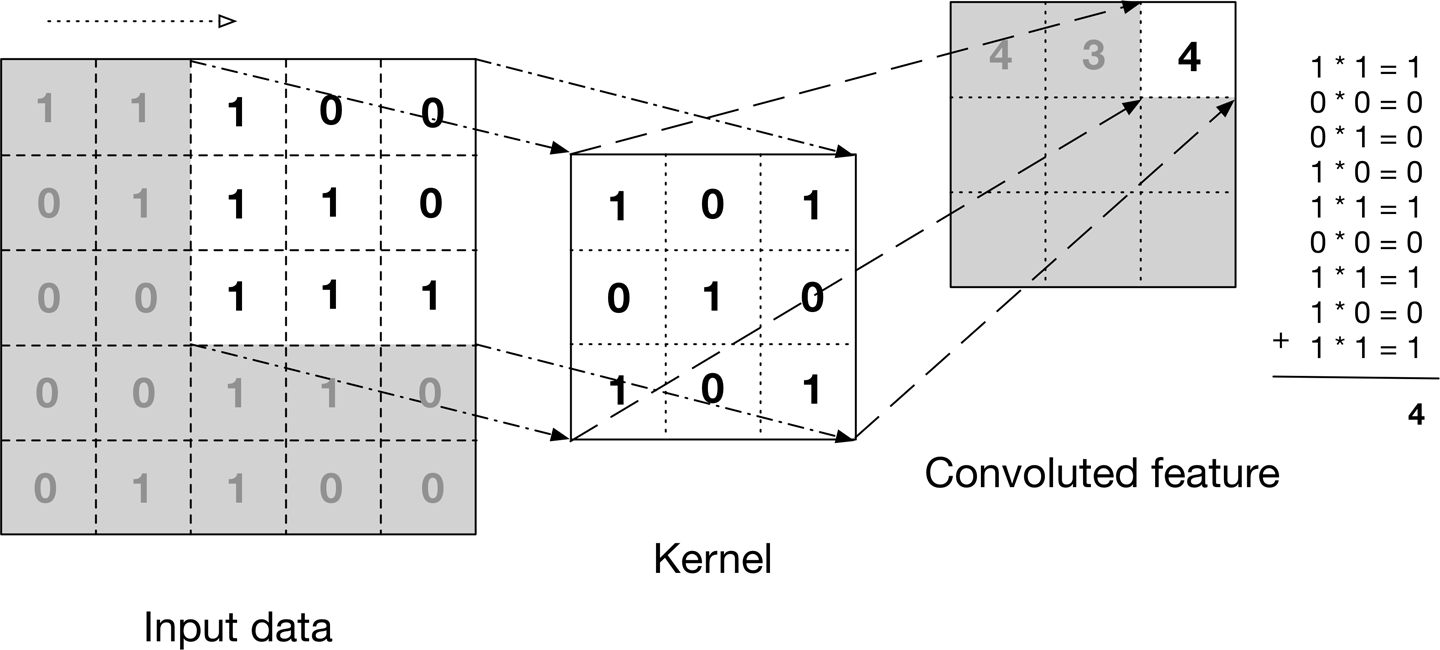
\includegraphics[width=.8\textwidth]{./images/illustrations/cnn}
    \caption{Concept of a convolutional layer. Source: Deep Learning by Josh Patterson, Adam Gibson}
    \label{fig:cnn}
\end{figure}


The connectivity pattern of sharing the same connectivity weights between all neurons in neighbouring layers is inspired by the visual cortex in the mammalian brain.
Mathematically, the operation can be approximated by a convolution operation, which gave the network architecture its name. 

While the name CNNs implies that all layers work with kernels the high level reasoning or classification task has to be done by at least one fully connected layer at the end of the network as shown in \ref{fig:typical-cnn}:


\begin{figure}[h]
    \centering
	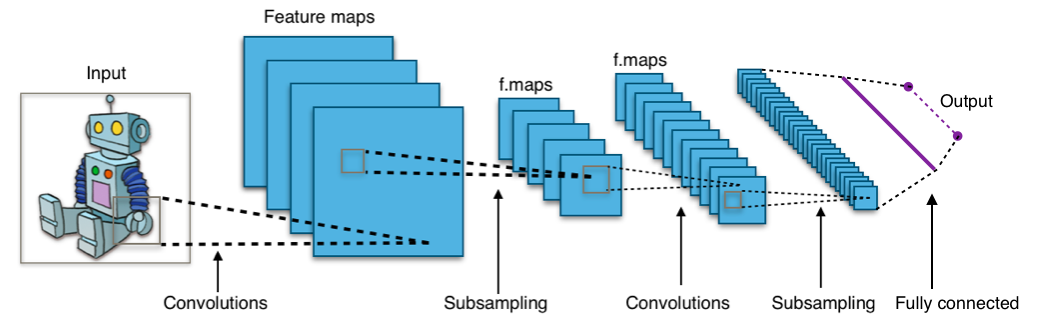
\includegraphics[width=.95\textwidth]{./images/illustrations/typical-cnn}
    \caption{Typical CNN architecture.\newline Source: \url{en.wikipedia.org}, by Aphex34; CC-BY-SA 4.0}
    \label{fig:typical-cnn}
\end{figure}


AlexNet is a famous example with 500,000 neurons in five convolutional layers \cite{AlexNet} that was a major breakthrough in the field of computer vision. It was submitted to the "Large Scale Visual Recognition Challenge 2012" which is commonly referred to as the annual olympics of computer vision.
During this competition AlexNet achieved a top-5 test error rate of 15.4\% on the 1.2 million images in 1,000 categories, while the second best entry only achieved an error of more than 26\% \cite{ILSVRC15}. 


This network consisted of five convolutional layers, includes dropout layers and employs three fully connected layers in front of the output layer. Instead of the conventional \texttt{TanH} activation function, \texttt{ReLU} made training more efficient.
Another innovation was the parallelization happening in the training. The authors split the networks layers into separate chunks that were trained on two independent graphic cards. The training still lasted six days, even though they were using two GTX 580 GPUs that were the most powerful solution on the market at that time.


Convolutional neural networks refers to any neural network with a convolutional layer.  These networks have achieved state-of-the-art results on many computer vision-related tasks, primarily because of their ability to "downsample" inputs while minimizing information loss.  It is because of this "downsampling" that these network are feasible to train, as opposed to a fully-connected network which has significantly more weights to train.  A convolutional layer is one that attempts to discover spatial relationships, aka filters, across neuronal inputs.
%[wtd describe + show graphs of convolutional layers].
This layer contains a set of filters or weight matrices that are convolved across the neuronal inputs, resulting in an output matrix called a feature map.  The weights of the filters are learned during training.  Typically these networks involve other spatial layers, such as max pooling layers, which directly downsample the neuronal inputs.

As some audio feature extraction methods output visual representations of the data that could be used for classification after some practice, it is likely that CNNs might play a vital role in this thesis. 

\subsection{Recurrent Neural Networks}

While CNNS solve the problem of dimensionality in terms of spatial relationships, RNNs do so in terms of sequential or temporal relationships.  Typically, to represent a temporal or sequential relationship inputs are stacked in a windowed-fashion.  However, this greatly increases the number of weights required at the input layer.  Therefore RNNs reduce the amount weights by allowing sequences to be passed in without requiring weights to be connected to these input features.


% http://colah.github.io/posts/2015-08-Understanding-LSTMs/



Nearly every animal has at least one form of memory and what happened in the past is always taken into consideration. In NNs however after completion of the training phase the past traditionally has no impact onto the result. 
In contrast, Recurrent Neural Network (RNNs) extend the idea by not only allowing feed-forward propagation but adding connections between units that form a directed cycle (loops) therefore allowing information to persist. 

\begin{figure}[h]
    \centering
	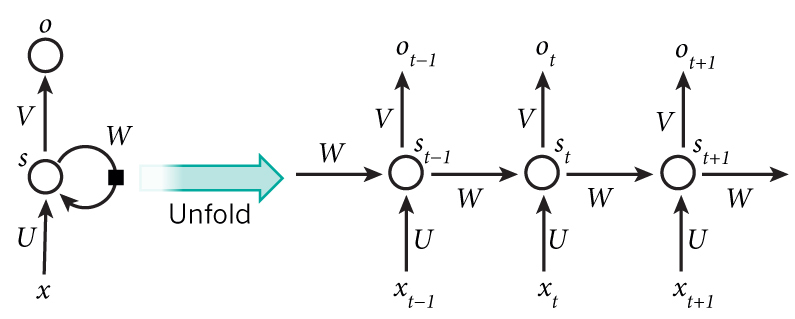
\includegraphics[width=.8\textwidth]{./images/illustrations/rnn}
    \caption{A recurrent neural network and the unfolding in time of the computation involved in its forward computation. Source: Nature}
    \label{fig:rnn}
\end{figure}


Adding this kind of internal memory has proven to be especially useful for tasks like speech recognition \cite{sak2014long} where due to the grammatical nature of human languages the meaning of heterographs (such as to, too and two) can almost always (and only) be determined by context.

The exact history of the first usage of RNNs is unclear. The english Wikipedia states that the first published version was the Hopfield-Network in 1982, however there is no citation to back this claim.

The concept of an RNN can be expanded to training a network without supplying specific labels to the training data but instead evaluating the network's performance through a reward function in certain intervals \cite{sutton1998reinforcement}. This process is known as reinforcement learning and was, for example, used to train the famous AlphaGo network on a trial-and-error basis by playing thousands of games against other instances of itself after it had reached the limit of proficiency achievable with supervised learning from 30 million moves by human experts \cite{alphaGo}.

%The simplest RNN is equivalent to a feed-forward network, where each cell's output $W$ 



%deep feed forward

%multi-dimensional long short-term memory 

%[wtd describe recurrent neural networks, cite original paper]

%[wtd include math and graphs of basic RNN structure]

%[wtd explain exactly the problem that RNNs solve (sequence and removing the need to include historical data in the inputs similar to how CNNs solve the problem of needing so many weights for the spatial input)]




\subsubsection{LSTMs}

One of the pitfalls of recurrent neural networks like the traditional single tanh layer as a repeating module is their practical difficulty with remembering information for a longer period of time. \cite{279181} showed that this is due to an inherent trade-off between efficient learning through gradient-descent and longevity of learned information and suggested that this problem might be solvable by modifying the optimisation algorithm or by employing a different method of optimisation altogether.

 Subsequently \cite{Hochreiter:1997:LSM:1246443.1246450} introduced a new cell architecture to solve the problem of vanishing or exploding error signals which the authors named LONG SHORT-TERM MEMORY. 
 Instead of a single neural layer each LSTM module contains four different ones that are connected through pointwise vector operations to interact  as a temporal storage.
 
\begin{figure}[h]
    \centering
	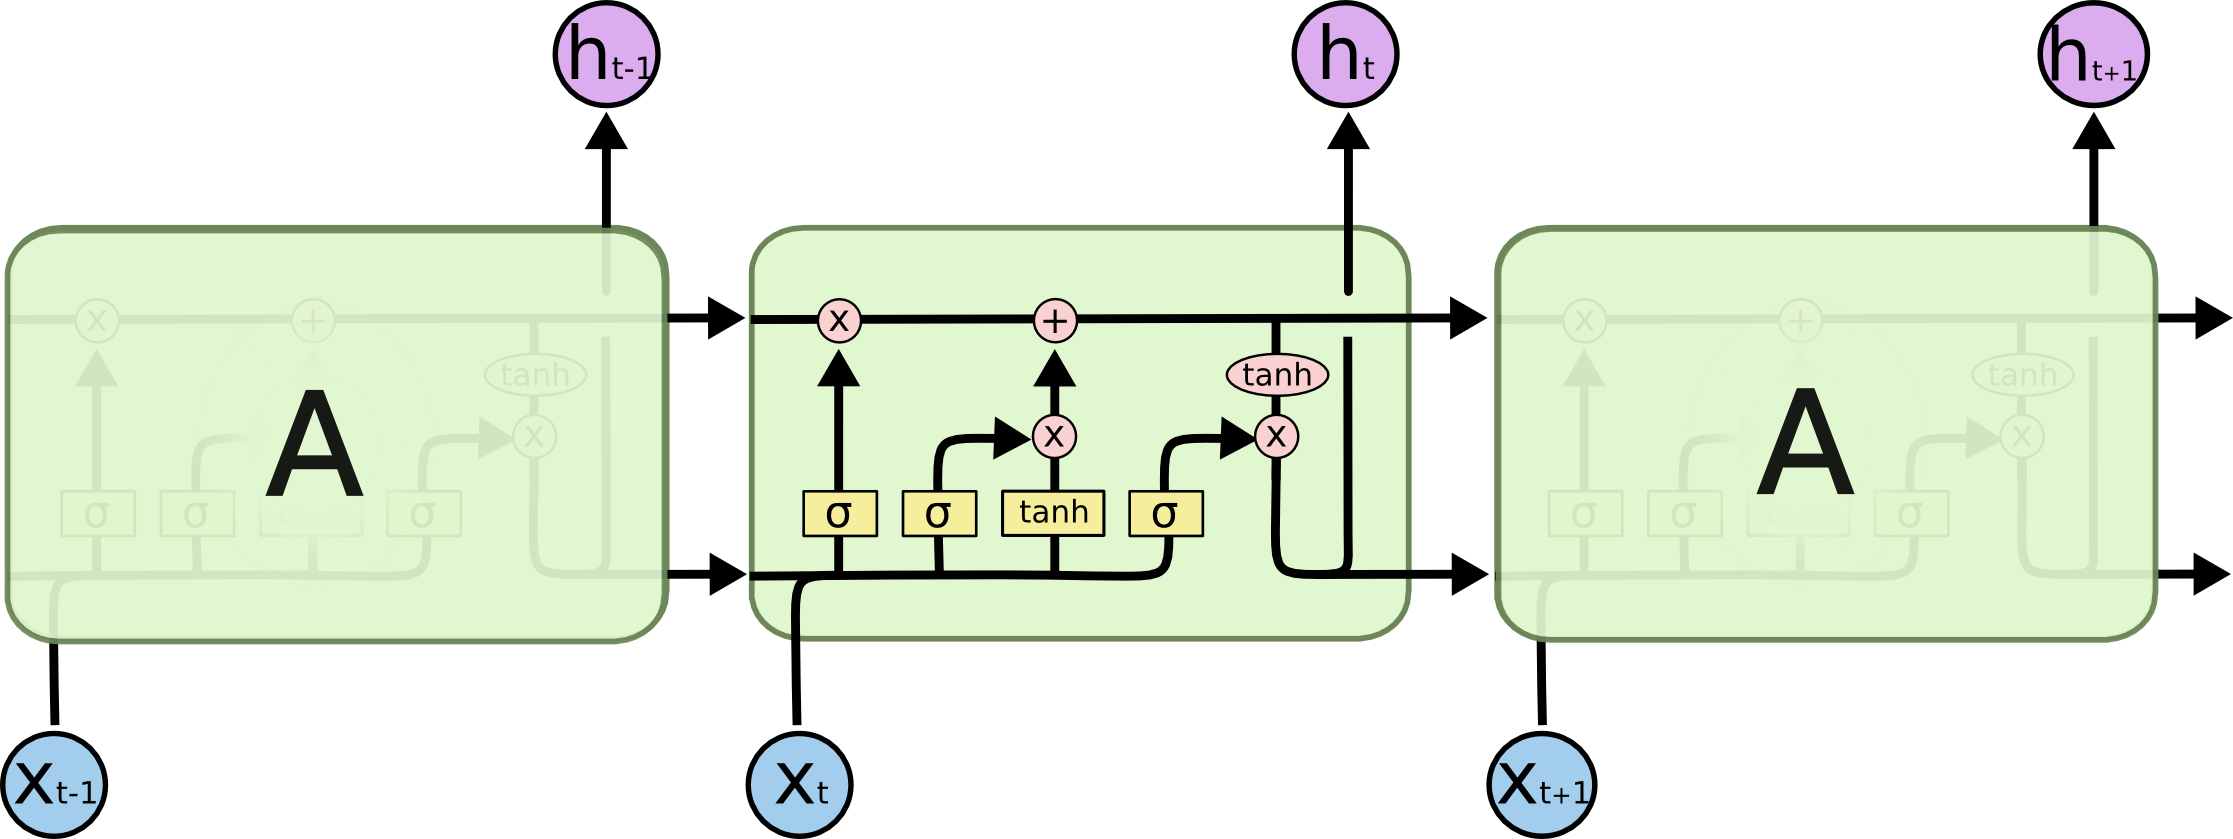
\includegraphics[width=.95\textwidth]{./images/illustrations/LSTM3}
    \caption{The repeating module in an LSTM contains four interacting layers. Source: \url{colah.github.io}. Reproduced with permission}
    \label{fig:mesh1}
\end{figure}

 
 Consequently, each module consists of an input vector $x_t$, an output  $h_t$, and an internal state vector $C_t$ which is preserved over time but can be modified by vector operations on data calculated by internal forget and input gates.
 
 % $+ V_{f} \circ c_{t-1} $ include state in forget operation?!
 The forget gate $f_t = \sigma (W_{f} * x_t + U_{f} * h_{t-1} + b_f)$ is calculated in each step and subsequently multiplied with the cell state $C_{t-1}$ where the value of $0$ (sigmoid minimum) would completely reset the cell state and the value of $1$ (sigmoid maximum) would entirely carry over the previous state's value.

In a similar fashion new information can be added to the cell state through an input gate $i_t$ that decides whether new input should be stored or not. Its result is then multiplied with a new candidate vector $\tilde{C_t} = \tanh(W_{c} * x_t + U_{c} * h_{t-1} + b_c)$. This final value is the new cell state $C_t = f_t \circ C_{t-1} + i_t \circ \tilde{C_t}$

The output is calculated by an output gate that considers the current cell state as well as the input and the previous output so that $h_t = tanh(C_t) \circ \sigma (W_{h} * x_t + U_{h} * h_{t-1} + b_h)$.

%While there are many different RNN architectures I have found the so called Long-Short Term Memory (LSTM) to be the most useful for the detection of driver frustration. % why?
%These are especially well suited to remembering information for a long period of time, where other RNNs like the traditional single tanh layer as a repeating module very often struggle \cite{Hochreiter:1997:LSM:1246443.1246450}.


LSTMs have been extremely successful in language processing and generation and related fields such as image captioning. With the advancement of GPGPU offering a much higher computational power regarding matrix multiplications LSTMs started to win competitions such as the "ICPR 2012 Contest on Mitosis Detection in Breast Cancer Histological Images" \cite{10.1007/978-3-642-40763-5.51}. Recently Microsoft Research announced that they had successfully built a conversational speech recognition system using a CNN-LSTM architecture that yielded a 5.1\% word error rate, achieving parity with human transcribers \cite{DBLP:journals/corr/abs-1708-06073}. The amount of success has been so stunning that Andrej Karpathy, Director of AI at Tesla and at that time Research Scientist at OpenAI published a blog post titled "The Unreasonable Effectiveness of Recurrent Neural Networks"\footnote{\url{http://karpathy.github.io/2015/05/21/rnn-effectiveness/}}.

While the original version of the LSTM introduced by \cite{Hochreiter:1997:LSM:1246443.1246450} has been very successful many researchers have  been working on further improving the effectiveness or reducing the required computational power for training to improve efficiency. A popular variation is the "Peephole LSTM" introduced with \cite{861302} where the sigmoid and tanh gates $f_t$, $i_t$ and $o_t$ also consider the internal state and which is the version erroneously described as the default implementation in the German Wikipedia\footnote{Permalink: \url{https://de.wikipedia.org/w/index.php?title=Long_short-term_memory&oldid=175151186}} as well as the GRU described in the next chapter.


\subsubsection{GRUs}


The GRU is a simpler recurrent cell introduced by \cite{DBLP:journals/corr/ChoMGBSB14}. The main difference is that it does not contain an internal state $C_t$ so that only the output $h_t$ is persisted over time and that it does not require an output gate. There is some debate whether the GRU is an independent RNN architecture or simply another LSTM variant. 

%the forget and input gates are replaced by a single update gate $z_t$.

\begin{figure}[h]
    \centering
	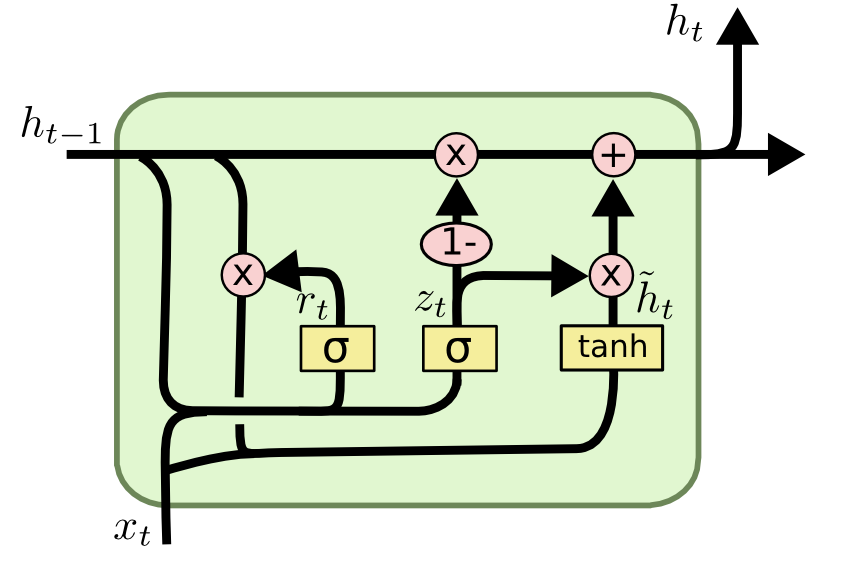
\includegraphics[width=.8\textwidth]{./images/illustrations/GRU}
    \caption{A GRU, as defined by \cite{DBLP:journals/corr/ChoMGBSB14}. Source: \url{colah.github.io}. Reproduced with permission}
    \label{fig:mesh1}
\end{figure}

While Wikipedia\footnote{Permalink: \url{https://en.wikipedia.org/w/index.php?title=Gated_recurrent_unit&oldid=829634771}} lists multiple variants (called types) that differ in the consideration of bias or the previous state within the gates, I was not able to find noteworthy advantages over the default version (named "fully gated" in the article) in literature.

At the time of submission the question whether there is a universal type of RNN cell that works best independent of context remains up for debate. When Google researchers did an empiric evaluation of more than ten thousand architectures in \cite{45473} they found that some variants might improve outperform both the standard LSTM as well as the GRU in certain but not all tasks. As the ration between resources and performance in my opinion currently favours the GRU I have decided to primarily focus on this architecture for this thesis.



\subsubsection{Attention Mechanisms}

\begin{figure}[h]
    \centering
	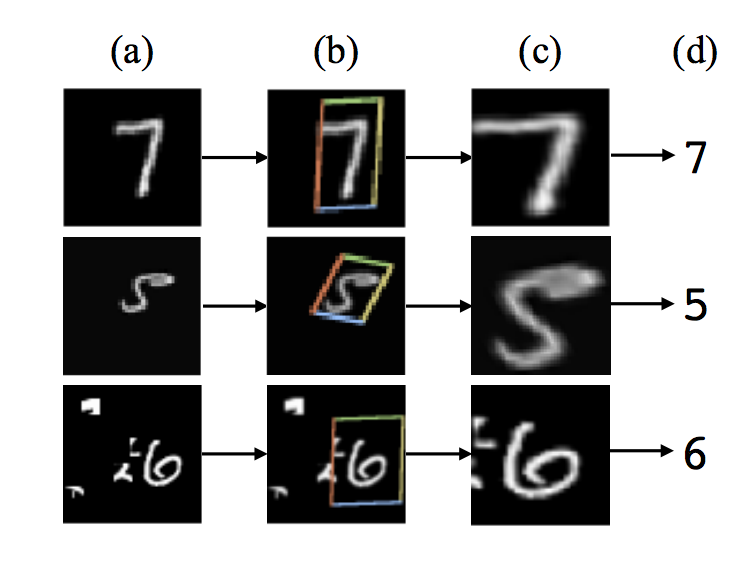
\includegraphics[width=.65\textwidth]{./images/illustrations/attention}
    \caption{The result of using a spatial transformer as the
first layer of a fully-connected network trained for distorted
MNIST digit classification in \cite{DBLP:journals/corr/JaderbergSZK15}.}
    \label{fig:attention}
\end{figure}


A very interesting recent discovery in the neural network architectures is that of attention mechanisms. OpenAI's research director Ilya Sutskever in an interview\footnote{\url{https://www.re-work.co/blog/deep-learning-ilya-sutskever-google-openai}} even went so far as to claim that "attention models, due to their simplicity and due to the fact that they work so well" would excite him the most in the field. It roughly mimics the concept of human attention (or focus) by allowing a neural network to "concentrate" on a specific area of input, and has produced state-of-the-art results in several machine learning tasks such as speech recognition or OCR of distorted content \cite{DBLP:journals/corr/JaderbergSZK15}. 

\begin{wrapfigure}{r}{0.45\textwidth}
    \centering
	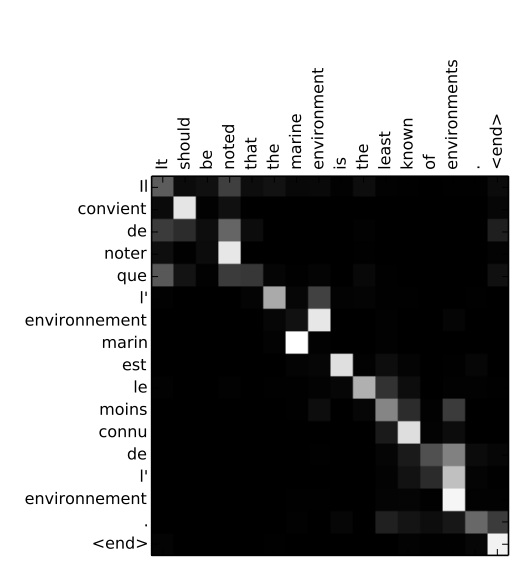
\includegraphics[width=.45\textwidth]{./images/illustrations/attention-bahdanau}
    \caption{Alignment of source and target language as visualised in \cite{DBLP:journals/corr/BahdanauCB14}}
    \label{fig:attention}
\end{wrapfigure}
This mechanism became famous because it caused a revolutionary breakthrough in the field of machine translation. Just like audio, classic translation algorithms usually relied on elaborate hand-crafted statistical models that were heavily depended on the input and output language.
The discovery of the attention mechanism however has enabled neural networks to outperform these. The method based on neural network differs significantly from traditional algorithms that relied on translating texts on a word by word basis or in chunks much smaller than a common sentence.
Neural machine translation on the other hand usually employs a sequence-to-sequence model \cite{DBLP:journals/corr/ChoMGBSB14}, which means a complete sentence is encoded into a content vector through an RNN and subsequently processed by a decoder, another RNN which generates the translated sentence in the target language. 

This seems counterintuitive as a human would not translate sentences of variable length in such an inflexible way. The attention mechanism solves this problem. Instead of having a universal fixed-length content vector that needs to hold all context in every step the decoder tells the encoder which content to process to which extent. As shown in \ref{fig:attention} a translation from french into english is attended almost sequentially due to the similar nature of the languages. Due to the high success and straight-forward implementation Google in the meanwhile even included a seq2seq translation with attention into their TensorFlow tutorial\footnote{\url{https://www.tensorflow.org/tutorials/seq2seq\#background_on_the_attention_mechanism}}.


% Attention beyond Machine Translation



\subsection{Deep Learning}

One of the primary advances in neural networks in the past several years has been the advent of deep learning.  Existing conceptually since the inception of neural networks, deep learning refers to network architectures with more than one hidden layer.  Conventionally speaking, a deep network is a network with many hidden layers, sometimes in the hundreds or thousans in \cite{DBLP:journals/corr/HeZRS15}. The discovery of adding more layers to a neural network to increase performance, however, has its own pitfalls.

For example, deep neural networks suffer from the problem of vanishing gradients \cite{Hochreiter:01book} and training time.  While previous approaches to conquering this problem have been somewhat successful \cite{DBLP:journals/corr/abs-1206-5533}, more advanced approaches have shown even greater success, for example normalization and regularization techniques, explained below.  Novel architectures such as deep residual networks \cite{DBLP:journals/corr/HeZRS15} have shown promise in this area as well.  Furthermore, the growing collection of larger annotated datasets and cheap, available processing power (such as GPUs and cloud computing), and the availability of open-source neural network toolkits have had major contributions to the success of neural networks as well \cite{tensorflow2015-whitepaper}, \cite{DBLP:journals/corr/SynnaeveNACLLRU16}. %TODO: cite open source dataset papers

What seems most interesting is that despite the remarkable successes researchers managed to achieve with deep learning the field is still very poorly understood. Especially in regards to the fundamentals there is no consensus in sight. While most people still try to understand and expand the field based on neuroscientific analogies others have argued that it has long transcended its biological origins in a similar way to aircraft designs that rarely copy birds nowadays. While an airfoil's lift can be fully explained and caluclated based on the physical principles of aerodynamics we however still lack a comprehensive explanation for deep neural networks. Consequently we can not always explain what our network are doing and especially it is especially difficult to understand what went wrong whenever an experiment fails.

This is why researchers have come up with other narratives. Christopher Olah, from whom I have gained most of my knowledge, has argued in an essay\footnote{\url{http://colah.github.io/posts/2015-09-NN-Types-FP/}}, which he only published on his blog, that deep learning is the intersection of algorithmic optimisation and functional programming. To illustrate this he has drawn many analogies between type theory and data representations in common networks, the concept of a neuron as a reusable abstractions, and multiple layers acting as chained functions transforming data. 


\subsection{Recent Advances in Neural Networks}

Up until 2010 neural network weights were usually initialised randomly before the weights were adjusted during training.  Contributing to the success of deep neural networks, several different initialisation schemes have been discovered like the He normal initialiser in \cite{DBLP:journals/corr/HeZR015} and the Glorot uniform initializer, also called Xavier uniform initialiser in \cite{pmlr-v9-glorot10a}.

For example, research into normalisation and regularisation has lead to faster training rates and higher accuracy, while preventing overfitting.  More specifically, batch normalisation\footnote{A good introduction to batch normalisation can be found here: \url{https://kratzert.github.io/2016/02/12/understanding-the-gradient-flow-through-the-batch-normalization-layer.html}} has shown to be greatly advantageous in speeding up the training of neural networks while reducing the amount of hyperparameter tuning \cite{DBLP:journals/corr/IoffeS15}. Batch normalisation however is inefficient whenever the batches do not consist of independent samples, such as in the UrbanSound8K dataset and introduces some extra overhead during training and network configuration.

% Bottom line, BN is definitely a very powerful tool to tackle existing problems but it should be noted that it does not come for free. First, BN introduces some overhead during training in terms of space, extra parameters, and time, for the data normalization. Second, layers in networks needs to be adjusted because BN is applied before the activation and third, a post-processing step is often required.

Even more recently, work has been done in the area of self-normalising networks 
% \footnote{A good introduction to self-normalisation is available at: \url{https://medium.com/towards-data-science/selu-make-fnns-great-again-snn-8d61526802a9}}
 that remove the need for batch normalisation and greatly increase accuracy and training speed in fully-connected neural networks. This is done by neuron activations that cause data to converge towards zero mean and unit variance \cite{DBLP:journals/corr/KlambauerUMH17}. To construct such a network neurons need to employ the SELU activation function described in \ref{selu}. A normal dropout method that during training sets random hidden layer's weights to zero with a certain probability (usually 50\%) to reduce overfitting interfers with mean and variance of the output and is therefore not suitable for the idea of self-normalisation.  
 The authors conclude that this is because, contrary to ReLU, the low variance limit of SELU is not zero. Therefore they subsequently introduce a modified technique which they have named "$\alpha$-dropout" where the weight of a dropped out neuron is instead set to $-\lambda\alpha$.



% Can maybe be expanded to page 35

\chapter{Public Urban Sounds Datasets}

\section{Urban Sound 8K}
The UrbanSounds8K dataset used for this research was published in 2014 with \cite{Salamon:UrbanSound:ACMMM:14}. It contains audio recording from the Freesound API, initially comprised 1302 recordings with the total length of 27 hours of audio and was manually labelled according to the Urban Sound Taxonomy created and introduced with the same paper. Labels span over 10 low-level classes in this taxonomy and offer an additional salience (foreground or background) classification.

\subsection{Creation}

The final audio samples have been provided by the authors publicly in the form of slices up to 4s long. Those were created by a 4s sliding window algorithm with a hop size of 2s and a limit of maximum 1000 slices per class. This results in a total of 8732 labeled slices or 8.75 hours of audio.

It is necessary to point out that the sliding window intentionally creates overlaps which result in the same audio information being present in up to two different slices. Additionally, due to the characteristics of urban sound, slices originating from the same original recording can have identifiable background or foreground sounds and other characteristics that can unintentionally be learned by the algorithm. %TODO: improve language

 This does not constitute a potential for error, as long as 
  slices from the same source are not diverted across training and validation set. The authors provide for that by splitting the data into 10 distinct folds intended for k-fold cross validation as a means of model verification.
  
  The files are provided in the losless .wav format. Parameters such as the sampling rate vary as they have not been changed from the original recordings.


%TODO: Overlap -> overfit
%[wtd explain advantages of this dataset, explain pitfalls, discuss other datasets and attempt to collect youtube horn dataset].

\subsection{Content}

As mentioned above, the dataset is labeled according to the Urban Sound Taxonomy(\cite{Salamon:UrbanSound:ACMMM:14}). The ten low-label classes present are air conditioner, car horn, children playing, dog bark, drilling, engine idling, gunshot, jackhammer, siren, and street music.

Unfortunately the occurences are unevenly distributed along the dataset, as shown in table \ref{tbl:urbansound8kdistribution}. 

\begin{table}[h]
\centering
\begin{tabular}{ll}
\hline
label & count \\
\hline
dog_bark & 1000 \\
children_playing & 1000 \\
car_horn & 429 \\
air_conditioner & 1000 \\
street_music & 1000 \\
gun_shot & 374 \\
siren & 929 \\
engine_idling & 1000 \\
jackhammer & 1000 \\
drilling & 1000
\end{tabular}
\caption{Amount of occurences per class in the UrbanSound8K dataset.}
\label{tbl:urbansound8kdistribution}
\par
\end{table}

The relatively low amount of car horns caused a problem, since the detection of various car horns was one of the AgeLab's main motivation. 

%TODO; Solution,Focus shift

\section{Creation of an own Car Horn Dataset}

That is why I have attempted to create an own dataset using recordings that are publicly available on youtube. The first step was to download traffic related videos; for reasons of applicability to other future tasks they were limited to the greater Boston area using YouTube's GeoSearch\footnote{A demo GUI is available at: \url{https://youtube.github.io/geo-search-tool/search.html}}.

\begin{wrapfigure}{r}{0.55\textwidth}
    \centering
	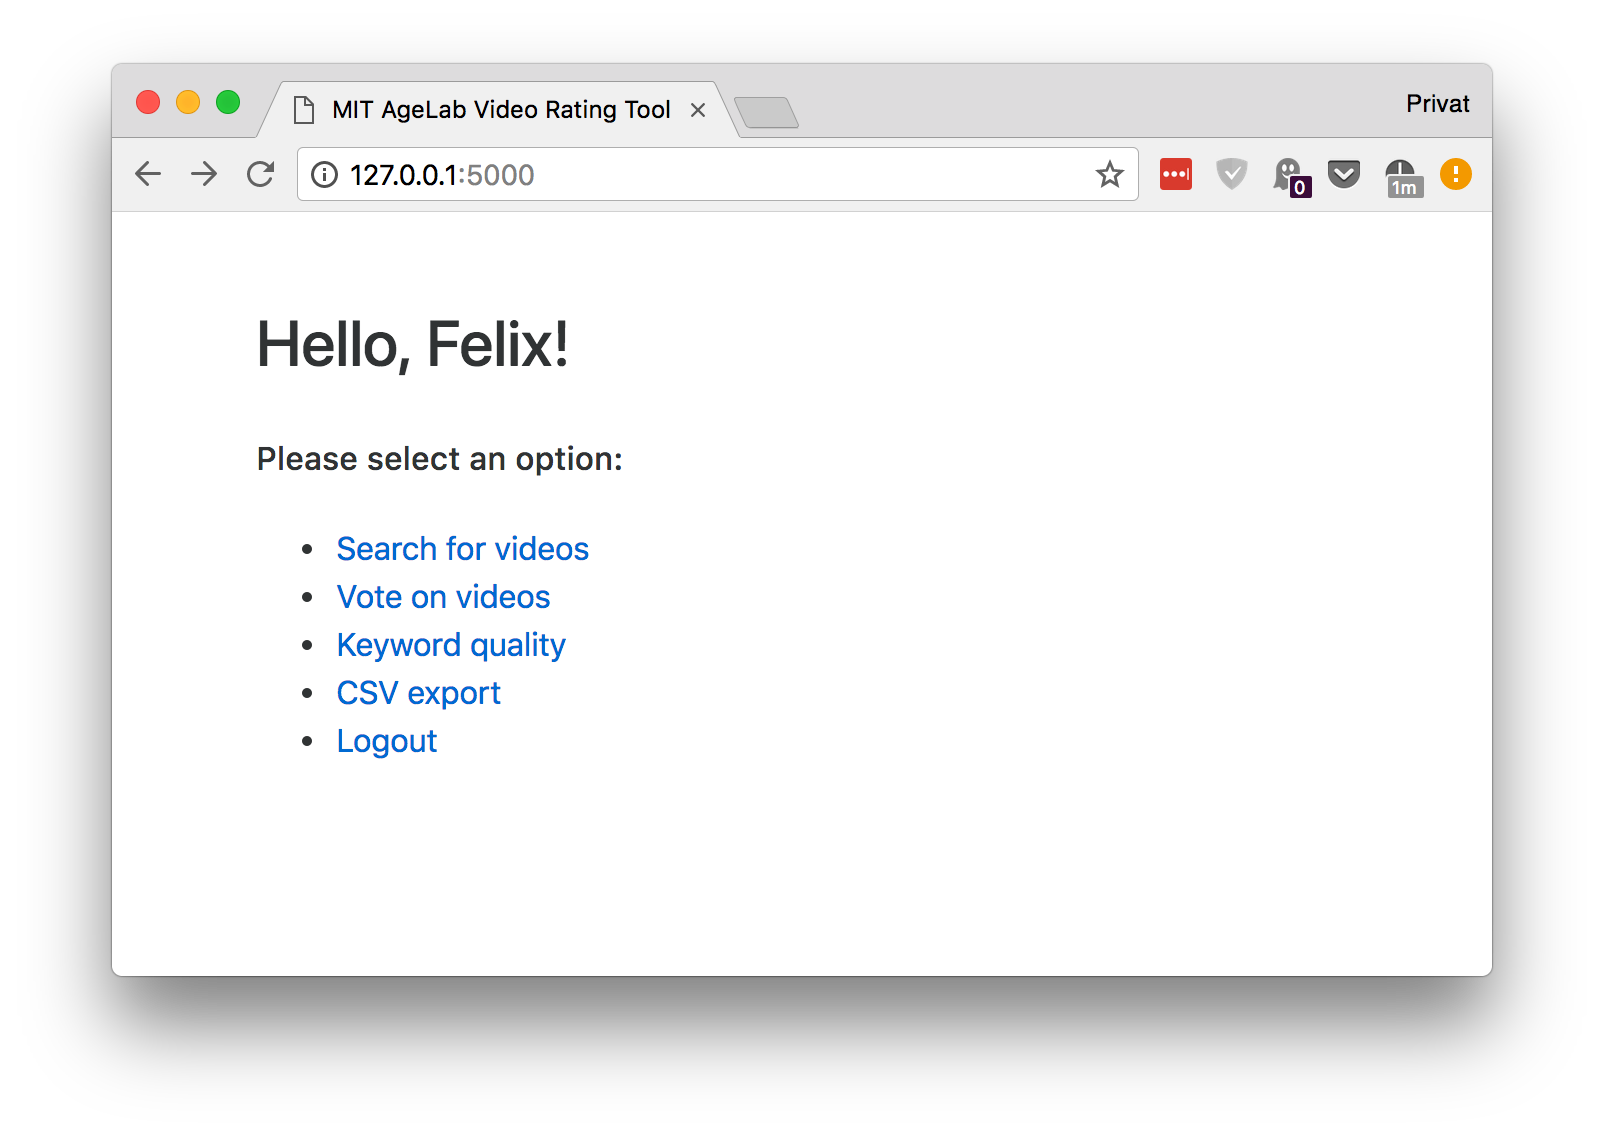
\includegraphics[width=.6\textwidth]{./images/illustrations/label}
    \caption{Index page of video search and labelling tool}
	\label{fig:label}
\end{wrapfigure}


To decide whether a video was useable I first had to build an annotation tool. This was implemented as a web application using the WSGI microframework Flask\footnote{\url{http://flask.pocoo.org/}} and the database abstraction layer SQLAlchemy\footnote{\url{https://www.sqlalchemy.org/}}. It provides a frontend for the YouTube search API which also logs each query to ease the search for specific keywords and geographical coordinates as well as to prevent redundant work. Later the videos can be previewed where the user votes whether each video is usable or not. In total the AgeLab team evaluated 800 videos during this step. What caught my eye was the high number of traffic video blogs (vlogs) that we uncovered, most with less than 100 views. 

After a CSV export all videos were downloaded and converted to wav using the youtube-dl\footnote{\url{https://rg3.github.io/youtube-dl/}} python api. In the next step the team listened to and manually annotated 9 hours of traffic noise using the open source Aegisub software, which is normally used to add subtitles to movies and tv shows. Different car horns were classified primary (foreground), secondary (background) or ignore (unusable, e.g. ambiguous or overlapping with other more prominent noise). That way the labels were encoded in the SubStation Alpha video subtitle format.


\begin{figure}[h]
    \centering
	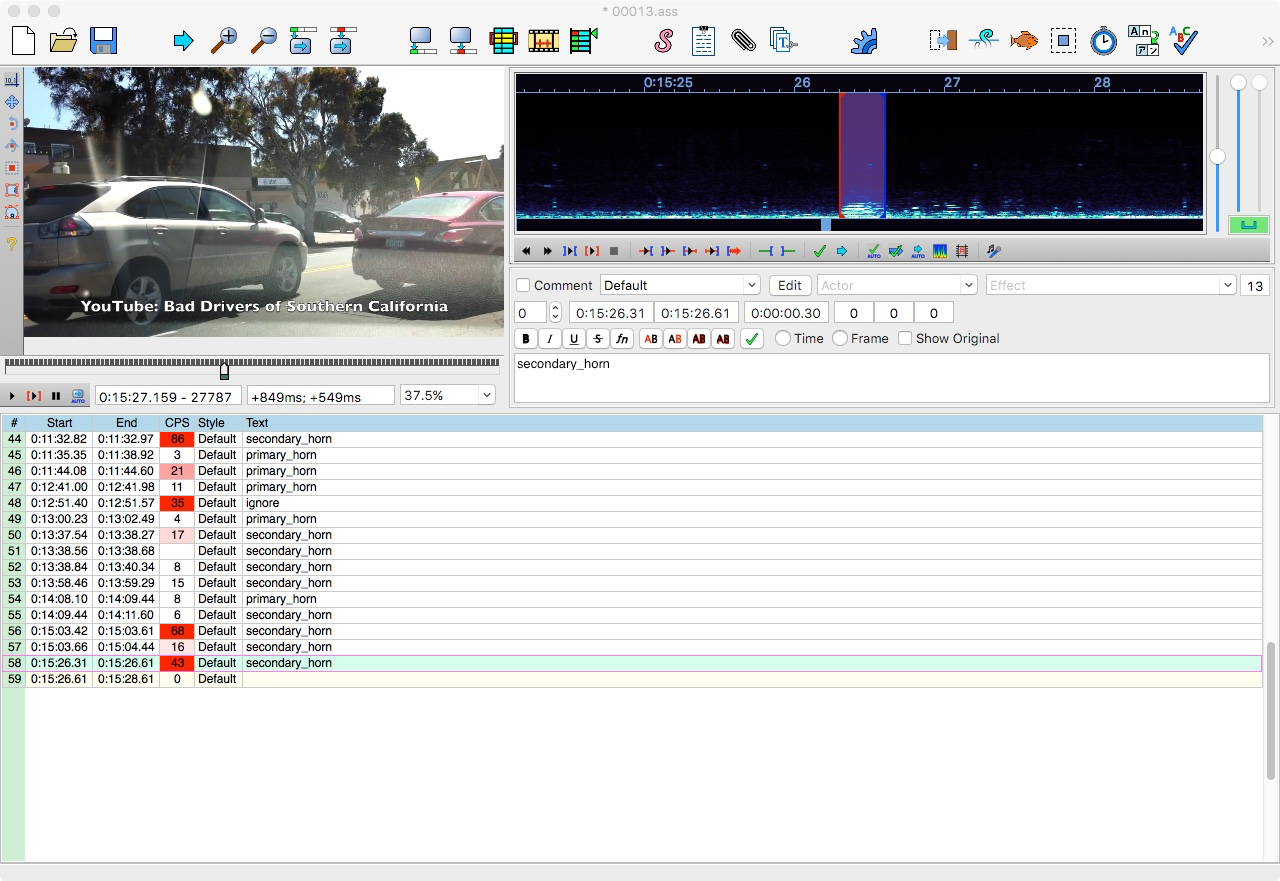
\includegraphics[width=.85\textwidth]{./images/illustrations/subt}
    \caption{Labelling car horns using Aegisub}
    \label{fig:subt}
\end{figure}



 The tags were later transformed into a single csv file with a python script. The result could be used to generate 1137 distinct audio clips through ffmpeg in 8 different folds which did not overlap files. While this method worked well there are two problem sources: the heavy editing of the vlogs, where voiceover often hushed the traffic sounds and the lossy audio compression done by youtube which is optimized for the human ear and might have removed information that could have been useful for our task.


\section{Google's AudioSet}

While I was working on this thesis the Machine Perception research team at Google published an own, versatile, audio dataset on March 5th, 2017 with the intent "to bridge the gap in data availability between image and audio research" \cite{45857}. It is simply named "Audio Set" and consists of 2'084'320 annotated video files totalling about 5.8 thousand hours of audio. Similar to my approach the content was extracted from youtube, however by owning YouTube Google was able to make heavy use of metadata, user behaviour, and context related searches results to ease classification.


\begin{wrapfigure}{r}{0.5\textwidth}
    \centering
    \vspace{-10pt}
	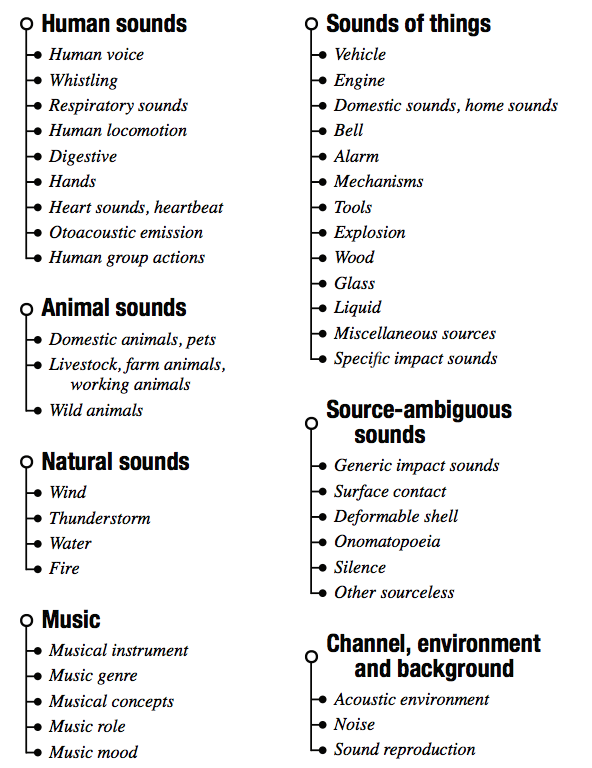
\includegraphics[width=.45\textwidth]{./images/illustrations/audioset}
    \caption{The top layers of the ontology introduced by \cite{45857}}
	\label{fig:audioset}
\end{wrapfigure}


While approximately half of the collection consists of music the amount of urban and indoor sounds is still at least two orders of magnitude higher than any previous dataset. As the dataset is no longer limited to a specific domain (such as urban sound) it required a new classification ontology which was introduced with \cite{45857} as well. This classification consists of 632 distinct categories that are hierarchically arranged up to a depth of 6 levels. The first two layers totalling 50 meta-classes are shown in figure \ref{fig:audioset} as displayed in the original publication. Eventually only 485 categories were released as some were ambiguous or did not contain more than 100 independent events.

The paper also introduced a simple neural network classification system which the authors describe as baseline. It is a fully-connected feed-forward network and achieves an average precision score of 31.4\% on 1 second frames. It is not stated which features are extracted or how the data is preprocessed. Another classifier from the same research group using CNNs and released as open source is described in chapter \ref{vggish}.


%lack of computing power in feature extraction

%detailed explanation of creation and labeling, baseline

%Paper: CNN architectures for large-scale audio classification

%e Fourier transform applying 25 ms
%windows every 10 ms. The resulting spectrogram is integrated into
%64 mel-spaced frequency bins, and the magnitude of each bin is logtransformed
%after adding a small offset to avoid numerical issues.
%This gives log-mel spectrogram patches of 96 × 64 bins that form
%the input to all classifiers. During training we fetch mini-batches of
%128 input examples by randomly sampling from all patches.

%Batch normalization 

%Adam optimizer

\newpage


\section{Feature Extraction}

As mentioned in the introduction, a raw audio signal consists of a high-dimensionality huge amount of data and is therefore not suitable as input for a learning algorithm without previous feature extraction.

This chapter contains visualisations of different features. It can be seen, that there is a distinct pattern per sound class that can easily be recognized by humans. It therefor is logical, that common image recognition networks should easily be able to lear these characteristics and be able to classify the audio files correctly along these characteristics.

statistical characteristics

show visulaisation among averages

% As noted in [13], the raw audio signal is not suitable as direct input to a classifier due to its extremely high dimensionality and the fact that it would be unlikely for perceptually similar sounds to be neighbours in vector space

% Thus, a popular approach for feature learning from audio is to convert the signal into a time-frequency representation, a common choice being the mel-spectrogram. We extract log-scaled mel-spectrograms with 40 components (bands) covering the audible frequency range (0-22050 Hz), using a window size of 23 ms (1024 samples at 44.1 kHz) and a hop size of the same duration. We alsoexperimented with a larger numbers of bands (128), but this did not improve performance and hence we stuck to the lower (and faster to process) resolution of 40 bands. To extract the mel-spectrograms we use the Essentia audio analysis library [20] via its Python bindings. Whilst we could use the resulting log-mel-spectrograms directly as input for the feature learning, it has been shown that the learned features can be significantly improved by decorrelating the input dimensions using e.g. ZCA or PCA whitening [18].

\subsection{Spectrogram}

\begin{figure}[H]
    \centering
	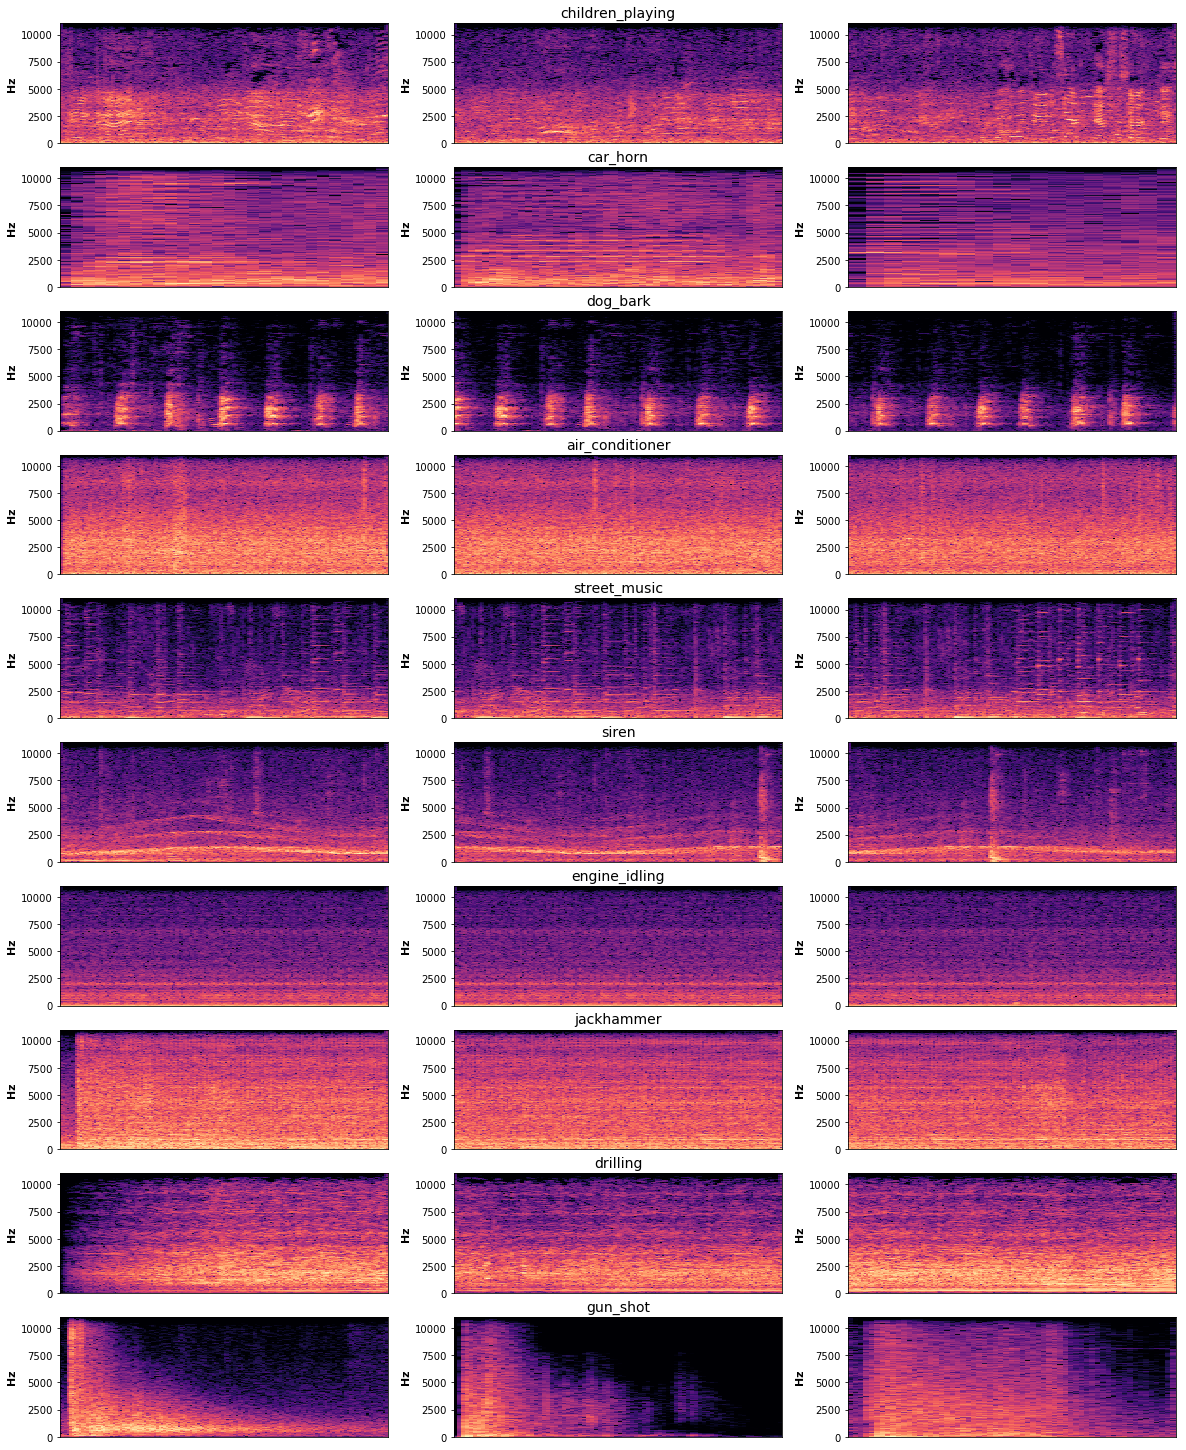
\includegraphics[width=.9\textwidth]{./images/features/spec-lin}
    \caption{Linear spectrogram of different audio classes}
    \label{fig:spec}
\end{figure}


\subsection{MFCC}


\begin{figure}[H]
    \centering
	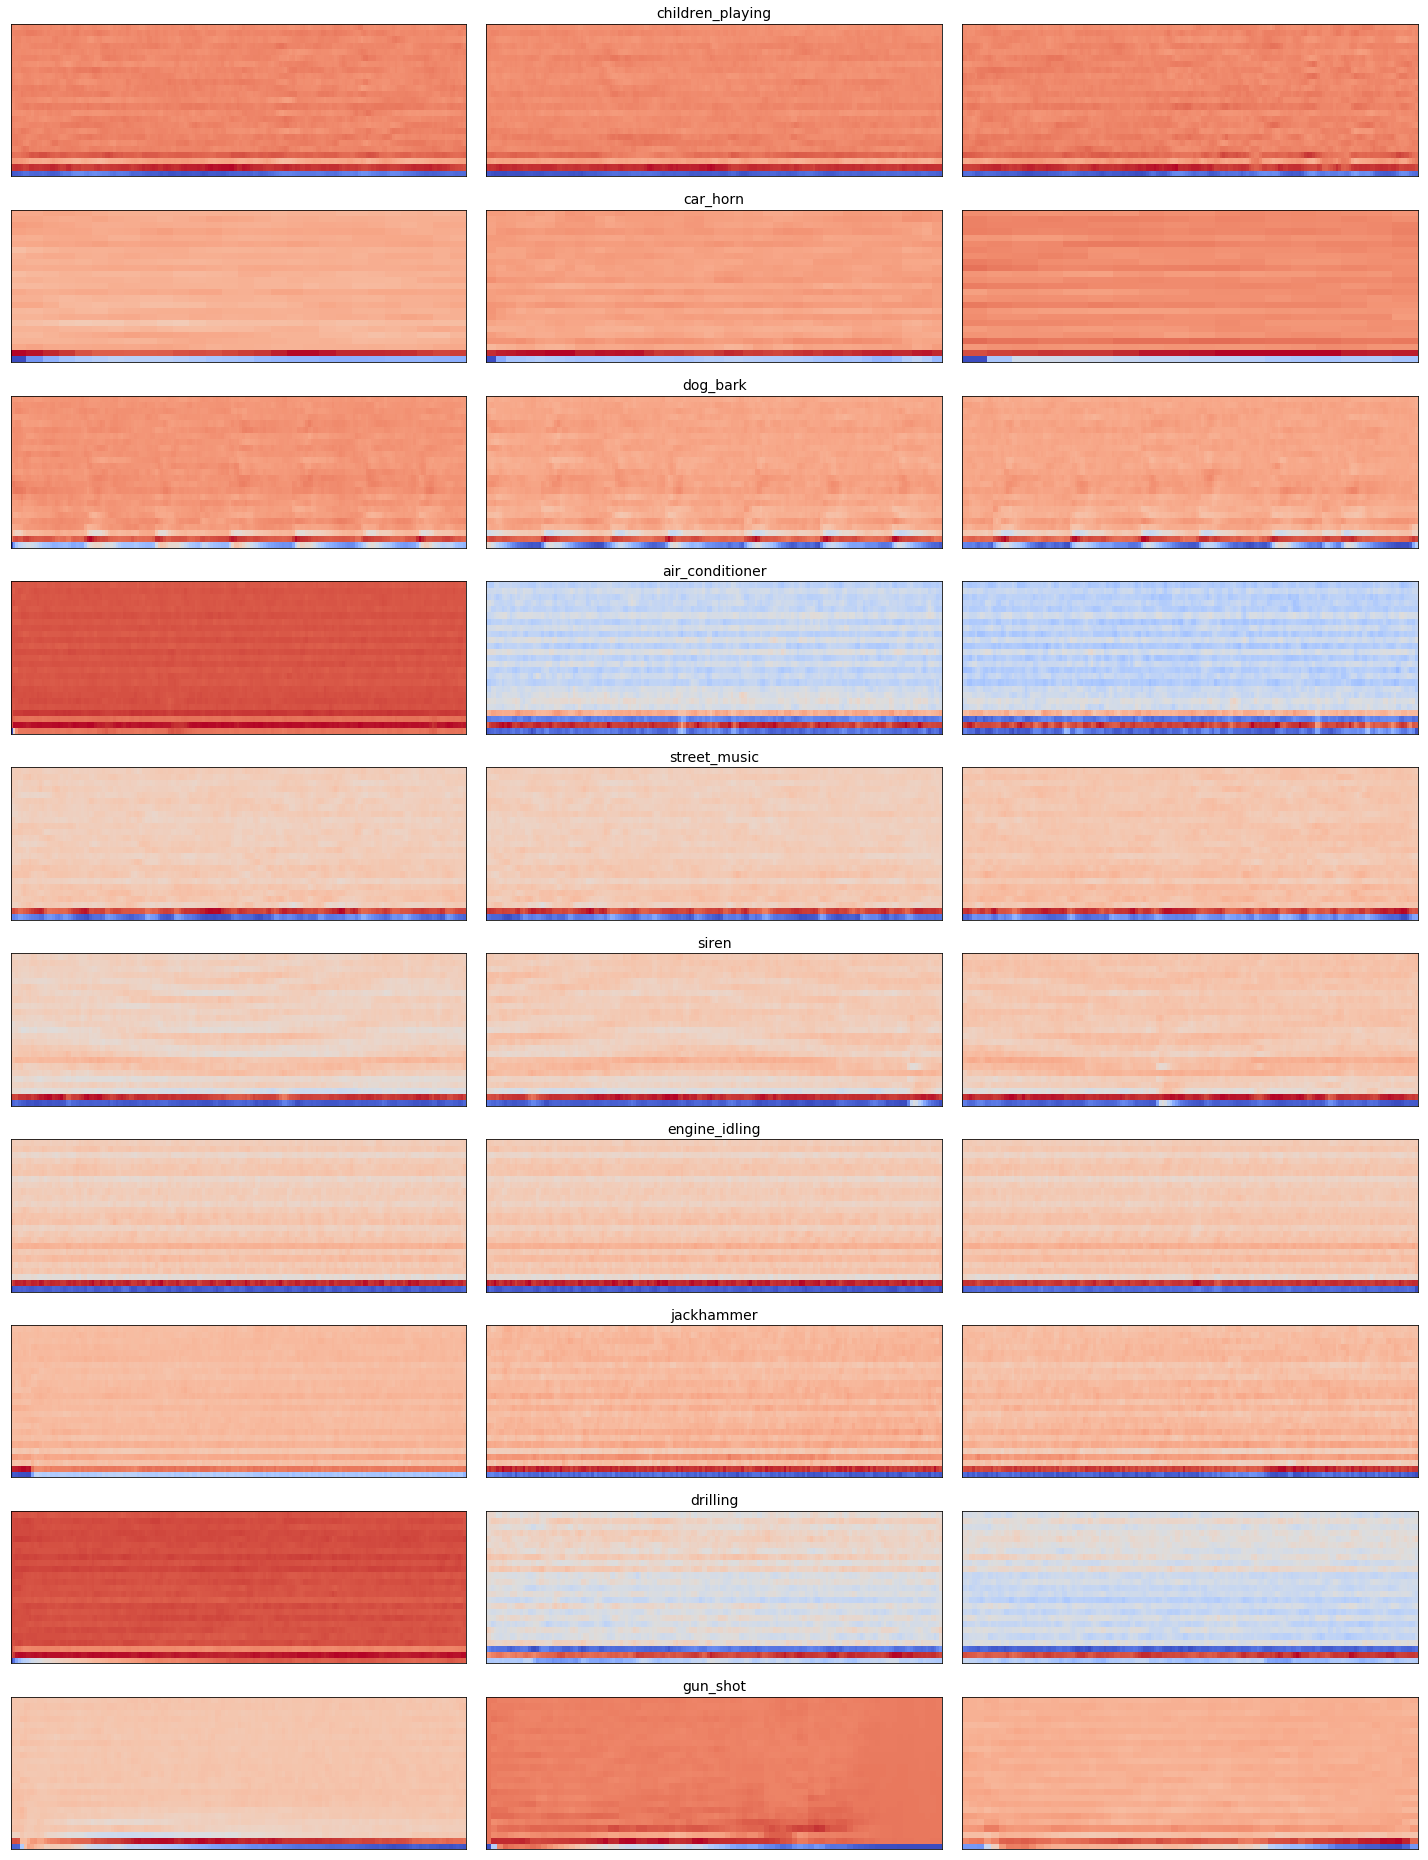
\includegraphics[width=.9\textwidth]{./images/features/mfcc-25}
    \caption{Visualisation of 25 Mel Frequency Cepstral Coefficients}
    \label{fig:mfcc}
\end{figure}



\subsection{Chroma}

\begin{figure}[H]
    \centering
	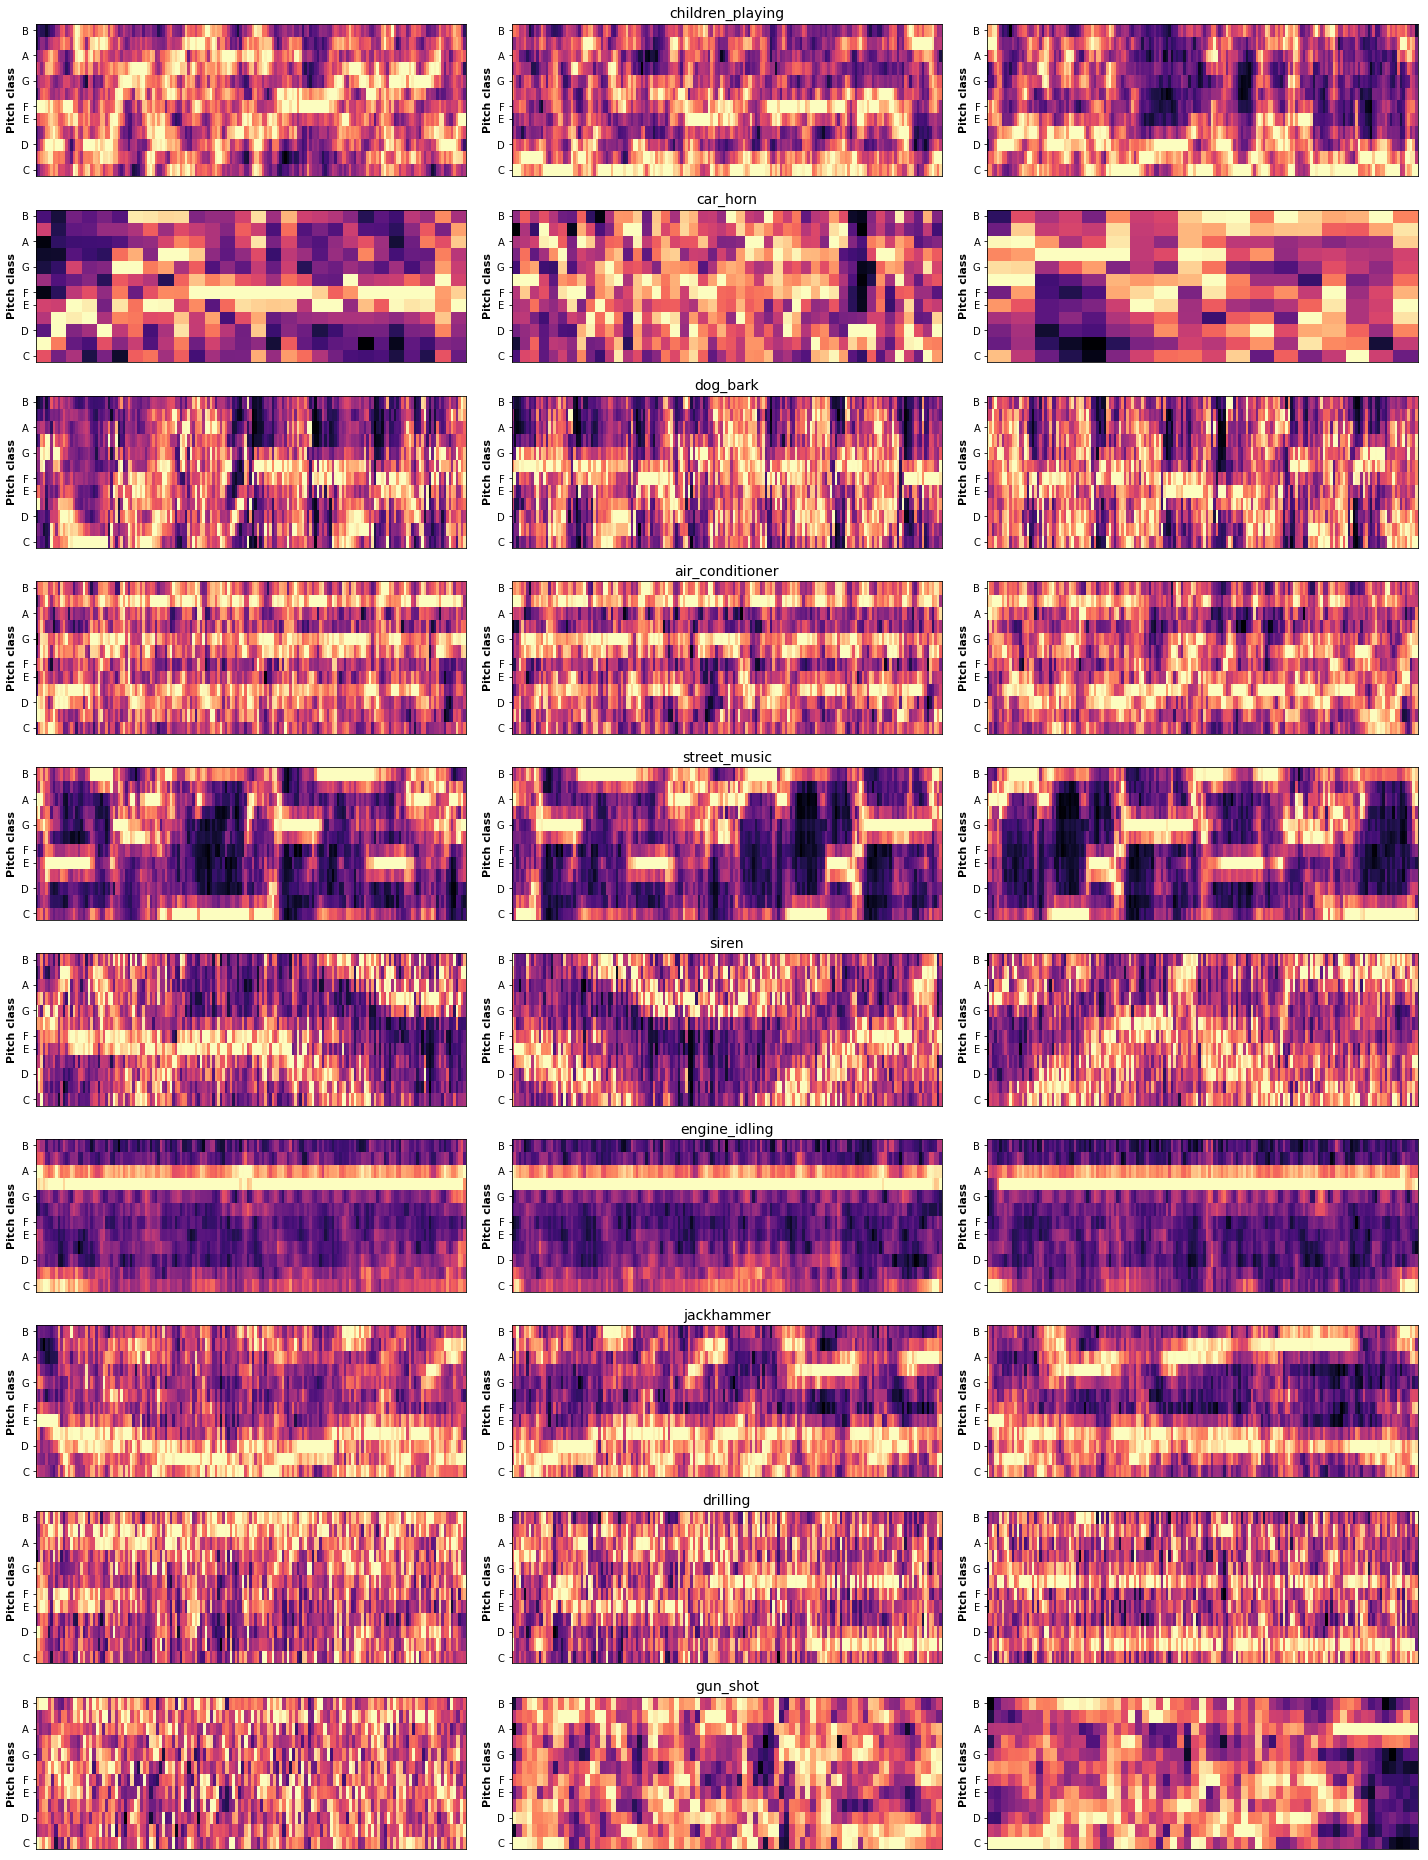
\includegraphics[width=.9\textwidth]{./images/features/chroma}
    \caption{Chromagram of different audio classes}
    \label{fig:chroma}
\end{figure}


Chroma shows little coherence, except for the classes engine_idling and siren.


\subsection{Quality Improvements}
While usually not being succesful with neural networks, there has been moderate success in the classification of bird songs and acoustic scenes using more traditional classification methods like the spherical k-means algorithm in the past. To improve classification accuracy, \cite{Coates2012} has shown that dimensionality reduction with PCA whitening over scaled features has significatnly increased accuracy. 
This indicates that extracted features of a mel spectrogram are still heavily correlated.

wtd noise

wtd temporal distortion


%[wtd describe what features are typically used in audio classification task]


% K MEANS

%[wtd describe what features were extracted by the SONYC team]

\chapter{Audio Classification Using GRUs and Attention Mechanisms}

[wtd discuss implementation]

\section{Feature Engineering}

[wtd discuss what inputs were used, and how they were shaped]

[wtd discuss any additional preprocessing done]

Spectrogram

MFCC (because Salmon et al) 

Log power average and variance over time -> CNN

LibRosa 

ESSENTIA




\newpage

Regression diagramm

First attempt Random Forest

Convolution matrix

accuracy: 69\%

SVM 72\%

accuracy diagram split by classes

\section{Network Architecture}

[wtd discuss exact nature of the architecture such as the layer, etc. include a graph, describe loss function]

Keras 

Attempt1: Feed Forward, recreation of Paper

Attempt2: CNN

Attempt3: RNN, GRU

adding attention


Unclear results -> If a CNN or a RNN is the better example remains open to debate.

Lower Accuracy in attempts 2 and 3: DATASET PROBABLY TOO SMALL FOR ANYTHING BESIDES FEED FORWARD


\newpage

\section{Training}

[wtd discuss batch sizes, number of epochs]

[wtd discuss train/test split, cross valdiation 10 fold?]

I have evaluated training across several optimizers including SGD + momentum, Adam, and RMSProp.  Results for each optimizer are included in figure [wtd link to figure showing training times and loss]

For training and modeling the neural network, we used Python with the Tensorflow and Keras libraries [wtd include Keras/tensorflow citations].

After the Hardware of my personal MacBookPro11,3 equiped with a 2,3 GHz Intel Core i7 (TensorFlow does no longer support GPU Acceleration on MacOS) reached it's limits, I managed to borrow a quad-core processor machine with an NVIDIA 1080 Ti graphics processor for network training from a friend free of charge.

Overall, training took a total of 4m 56s on this machine.

\subsection{The Problem of Overfitting}

Other approach: https://github.com/aqibsaeed/Urban-Sound-Classification

When I used his code and

Overfit, broke test/train folds, 

\newpage

\subsection{k-fold Validation}


SCORE Matrix


\newpage

\section{Results}

[wtd results table]

Overall, I was not able to achieve better than previously publsihed results on the SONYC urban sound classification dataset using LSTMs with attention mechanism.

[wtd discuss pitfalls]

\chapter{Other Approaches to Audio Recognition}

\section{VGGish model}
\label{vggish}

Source Code available

https://github.com/tensorflow/models/tree/master/research/audioset

Hershey, S. et. al., CNN Architectures for Large-Scale Audio Classification, ICASSP 2017

TODO try this model

\section{Comparing Gradient Boosting to GRUs and Attention}

In addition to the deep neural network approach, an attempt to use gradient boosted trees, using the xgboost library \cite{DBLP:journals/corr/ChenG16} to achieve similar results.  As mentioned, gradient boosting has been very successful in classification tasks involving a small input dimensionality.

\newpage



\section{Attempted Recreation of NYU Papers}

After receiving rather mediocre results on the SONYC dataset with my own network I have attempted to improve my own undestanding by recreating the papers published by the same team that provided the SONYC dataset.

There has been a community of amateurs on GitHub that have attempted to build projects on the UrbanSound8K dataset. https://github.com/aqibsaeed/Urban-Sound-Classification



For each experiment we report the average accuracy across all 10 folds.

[wtd differences in audio libraries and sklearn]

[wtd why were most results no reproducable]

Differences in Essentia and LibRosa, reference Chapter 2

%Scattering


ScienceMag Publication: Missing data hinder replication of artificial intelligence studies

Other user's attempt to replicate: https://github.com/cyrta/UrbanSounds

Speech and Music Technology Researcher Pawel Cyrta (ex Samsung)

Others have given up early or made significant mistakes

ReScience Project


\subsection{A Dataset and Taxonomy for Urban Sound Research}

In this paper \cite{Salamon:UrbanSound:ACMMM:14} the UrbanSound8K dataset is initially introduced. The authors in detail explain the creation (section three) and their proposed taxonomy (section two). At this point  our interest is focused on chapter four where an experimental setup for feature extraction and classification is discussed. It is also highlighted that this was about a baseline approach not aimed at an optimal configuration.

The features used for training are 25 Mel-Frequency Cepstral Coefficients (see \ref{MFCC}) computed on slices in the length of 23.2 ms with 50\% overlap. While the calculation is done using 40 Mel bands up to 22.05 kHz only the first 25 coefficients are actually used. As the length of each sound file is up to 4s, the results are transformed into a constant feature vector of dimension 225 by extracting 9 different statistical values per coefficient over time such as minimum, maximum and mean.

The feature vector is used to train different machine learning algorithms: decision tree (J48), k-NN (k = 5), random forest (500 trees), support vector machine (radial basis function kernel), and a baseline majority vote classifier (ZeroR). Unfortunately no further details on the hyperparameters are given. The authors conclude that there is a tie between the classifiers SVM and random forest at an accuracy of approximately 0.7.

I have tried to recreate the results of these two classifiers through Python's scikit-learn \cite{scikit-learn}. Unfortunately the attempt was rather unsuccessful. Even after experimental tuning, which included the reduction of \texttt{n_estimators} to 85 and increasing the \texttt{min_samples_leaf} to two or four in the random forest and excessive experimentation with the gamma value and different kernels for the SVM the accuracy never exceeded .64. These results are already questionable as these optimisations were done using the same k-fold validation technique used to measure the accuracy and there was no separate data set for hyperparameter tuning.
 
A source of error in my approach might be that the feature extraction in the original paper was done using the ESSENTIA library \cite{bogdanov:Essentia:ACMMULTIMEDIA13} while I attempted a recreation using librosa for compatibility reasons. 

\subsection{Unsupervised Feature Learning for Urban Sound Classification}

The subsequent paper \cite{7177954} is not focussed on the dataset anymore but on tradition machine learning approaches on the data. 

Essentia via Python Binding

40 MFCC

temporal dynamics

The data is decorrelated by using prinicpal component analysis (PCA) whithening. This feature is available in sklearn.

n_components = 0.99

svd solver unknown



Multi step approach:

Spherical k-means per audio file

1000 centroids

Pooling

Random forest



version of k-means not in sklearn. spherecluster? pip package

UNABLE TO IMPLEMENT


\newpage


\subsection{Deep Convolutional Neural Networks and Data
Augmentation for Environmental Sound
Classification}

no validation set


recreated network architecture exactly as described


methodological error: hyperparameters tuned on test set

dataset too small?





\chapter{Conclusion}

[wtd include results table of approaches to this dataset]

[wtd explain possible explanations for the results of our approach]

[wtd discuss problem with audio classification task]

It has been shown that most likely one of the primary reasons audio classification is such a difficult task is due to the lack of available data.  Therefore, as the amount of labeled audio classification datasets increases (such as in genre classification [wtd cite stanford audio classification paper]), it is likely predict there will be an increase in performance in this area.

